%
% Physical Architectures For Quantum Computing
%

\section{Physical architectures for quantum computing} \label{sec:archs_QC} \index{Physical architectures}

The models for quantum computation introduced in the previous section are abstractions of algorithms in terms of elementary operations. But elementary operations must ultimately be physically realised. There are countless physical architectures for realising quantum computations, far too many to describe here, each with their own advantages and disadvantages, and it is far from clear which physical architecture(s) will ultimately win the quantum race.

Here we will summarise some of the physical architectures most applicable to networking. Since we reasonably anticipate that future quantum networking will be optically mediated, we focus on pure-optical and hybrid-optical architectures, on the basis that these will naturally lend themselves to optical interfacing.

%
% Universal Linear Optics Quantum Computing (KLM)
%

\subsection{Universal linear optics (KLM)} \label{sec:KLM_univ} \index{Universal linear optics quantum computation}\index{Knill-Laflamme-Milburn (KLM)}

With single-photon encoding of qubits in the quantum network, the obvious architecture to implement quantum computation is linear optics quantum computing (LOQC) \cite{bib:KLM01} (KLM), since the states being processed by the computer are of the same form as the states traversing the network. See \cite{bib:Kok05, bib:KokLovettBook} for excellent introductions to this what has become a very broad and exciting field.

LOQC allows universal quantum computing to be implemented using single-photon polarisation or dual-rail encoding, with only linear optics interactions, i.e beamsplitter/phase-shifter networks \cite{bib:Reck94}, with the addition of quantum memory, and fast-feedforward, whereby some photons are measured, and the remaining part of the optical circuit is dynamically reconfigured based on the measurement outcomes. The former is readily available technology today, and elementary demonstrations have been performed \cite{bib:OBrien03, bib:UniversalLOOBrien}, but the latter two have proven to be somewhat more challenging.

Originally it was believed that universal optical quantum computation, specifically the implementation of two-qubit entangling gates (such as CNOT or CZ gates), would require extremely (and unrealistically) strong optical non-linearities that implement a non-linear sign-shift (NS) gate,
\begin{align} \label{eq:NS_trans}\index{Non-linear sign-shift (NS) gate}
NS: \alpha\ket{0}+\beta\ket{1}+\gamma\ket{2}\to\alpha\ket{0}+\beta\ket{1}-\gamma\ket{2},
\end{align}
in the photon-number basis, up to normalisation (which is determined by the post-selection success probability). That is, it applies a $\pi$ phase-shift to only the $\ket{2}$ component of a photon-number superposition. The breakthrough result by KLM demonstrated that this is in fact not the case at all. Instead, the NS gate can be implemented non-deterministically using post-selected linear optics. Two such NS gates allow the construction of a single CZ gate. The construction of the KLM NS and CZ gates are shown in Figs.~\ref{fig:KLM_gate} \& \ref{fig:KLM_explain}. Equivalently, a CNOT gate may be trivially constructed via conjugation by Hadamard gates, based on the identity \mbox{$\hat{H}\hat{Z}\hat{H}=\hat{X}$}.

\begin{figure}[!htb]
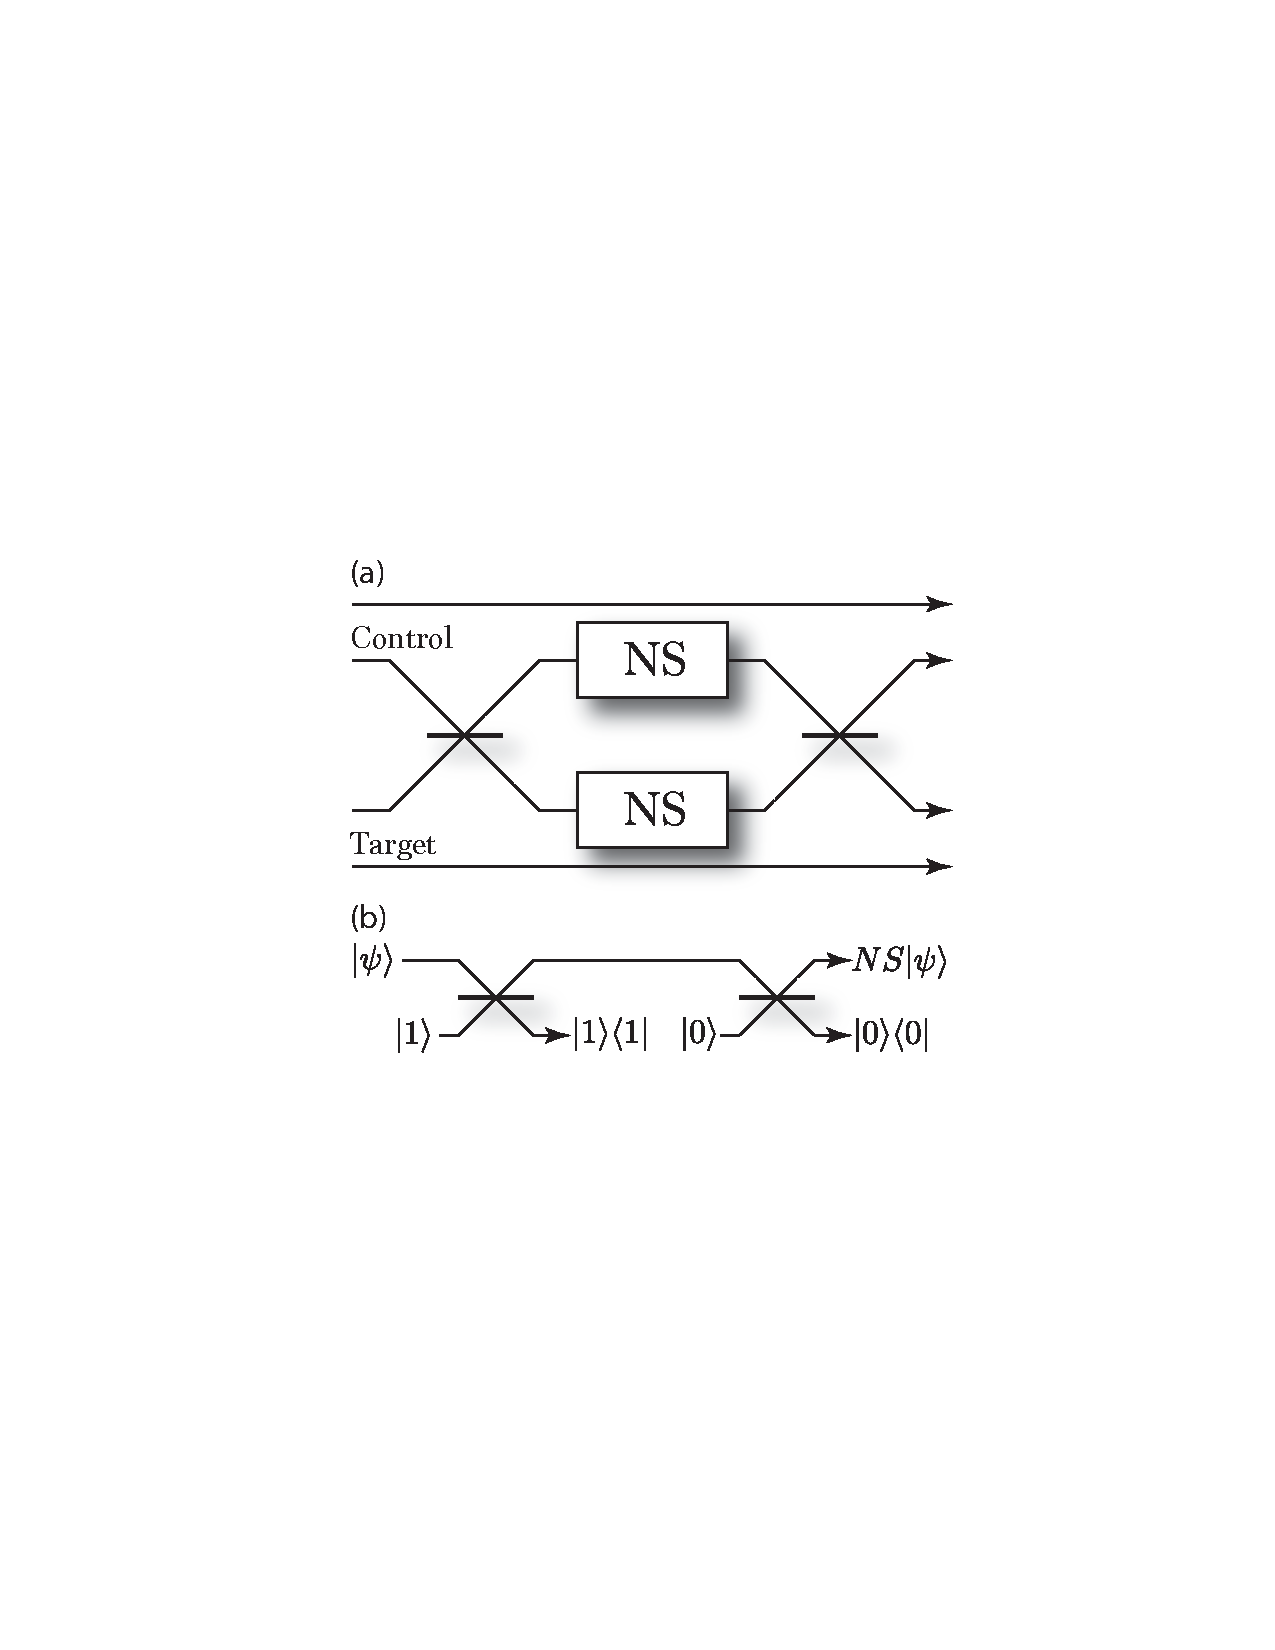
\includegraphics[width=0.8\columnwidth]{KLM_gate}
\caption{(a) A KLM CZ gate, employing dual-rail encoding, constructed from two non-linear sign-shift (NS) gates, which apply a $\pi$ phase-shift to only $\ket{2}$ terms in the photon-number basis. (b) Construction of the non-deterministic linear optics NS gate. Two ancillary states -- one $\ket{1}$ and one $\ket{0}$ -- are employed, and two photo-detectors post-select upon detecting $\ket{1}\bra{1}$ and $\ket{0}\bra{0}$ respectively. The beamsplitter reflectivities in (a) are 50:50, and in (b) chosen such that the amplitudes obey Eq.~(\ref{eq:NS_trans}).}. \label{fig:KLM_gate} \index{Knill-Laflamme-Milburn (KLM)}\index{Non-linear sign-shift (NS) gate}
\end{figure}

\begin{figure}[!htb]
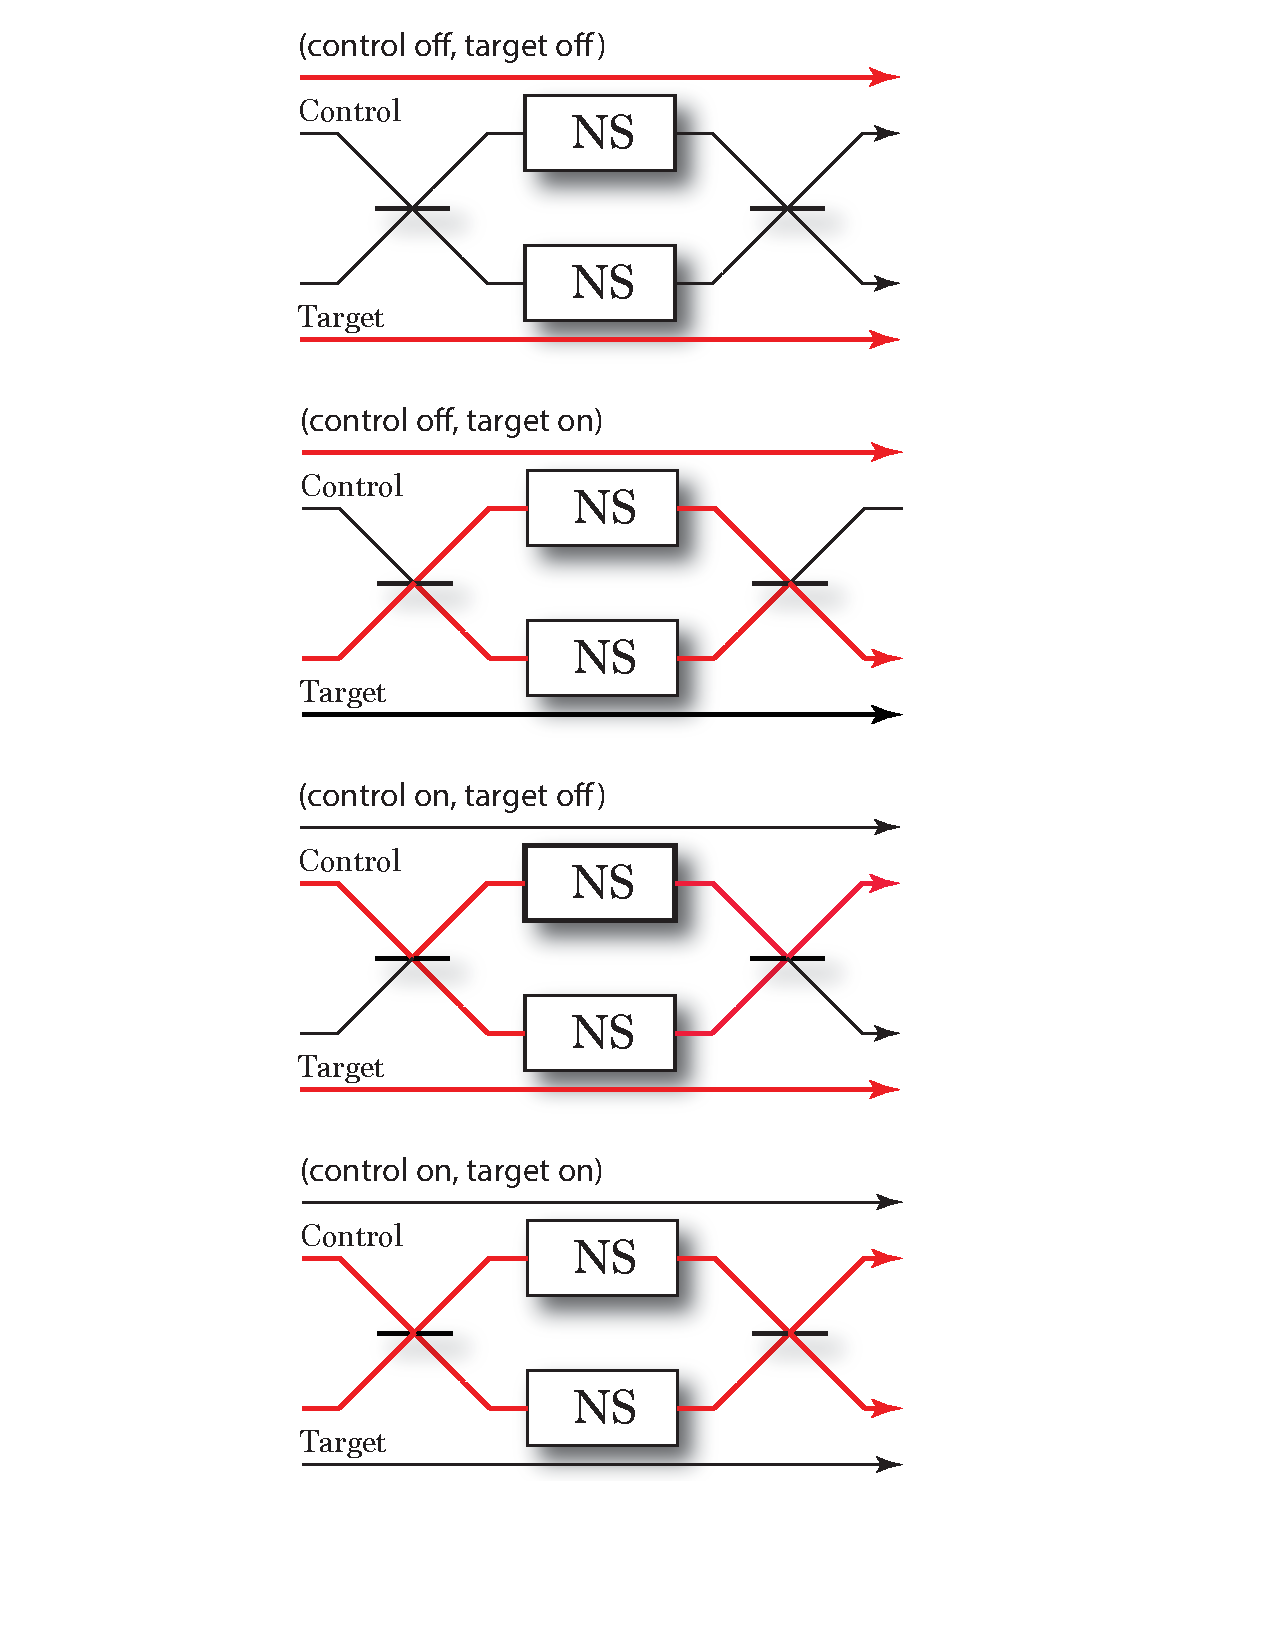
\includegraphics[width=0.9\columnwidth]{KLM_optical_paths}
\caption{Evolution of the four logical basis states through the KLM CZ gate. The NS gates do nothing in the first three cases, since they are operating only on vacuum and single-photon terms, which are left unchanged by the NS gate. In the last case, where both control and target are on, HOM interference results in photon bunching after the first beamsplitter, thereby creating two-photon terms. These terms inherit the $\pi$ phase-shift from the NS gate transformation, after which the final beamsplitter reverses the HOM photon bunching, yielding the same logical basis state with an acquired $\pi$ phase-shift.}. \label{fig:KLM_explain} \index{Knill-Laflamme-Milburn (KLM)}\index{CZ gate}
\end{figure}

Clearly this non-determinism is of immediate concern, since concatenating multiple gates would have exponentially decreasing success probability, making the protocol inefficient -- if the probability of a single gate succeeding is $p$, and we require that a circuit comprising $n$ of them all succeed, the success probability is clearly $p^n$.

The first key observation then is that gate teleportation can be used to shift this non-determinism to a resource state preparation stage, as described in detail in Sec.~\ref{sec:teleport_gate}. However, this is not the end of the story, since gate teleportation requires Bell state projections, which are themselves non-deterministic using purely linear optics (either using PBSs or CNOT gates). --- \textit{Ignotum per ignotius}.

The final insight provided by KLM is that by concatenating these non-deterministic CNOT gates, we can inductively build up higher-level CNOT gates with ever increasing success probabilities, asymptoting to unity with high-depth (but polynomial) concatenation. By combining these key insights, KLM were able to show that near-deterministic CNOT gates can be constructed using an efficient resource overhead, thereby enabling efficient universal quantum computation\footnote{Note that all single-qubit gates are trivially and deterministically implemented using wave-plates or beamsplitters, for polarisation or dual-rail encoding respectively. Thus, we need only concern ourselves with the challenges associated with implementing two-qubit entangling gates.}. A sketch of the general KLM formalism is shown in Fig.~\ref{fig:KLM_protocol}.

\begin{figure}[!htb]
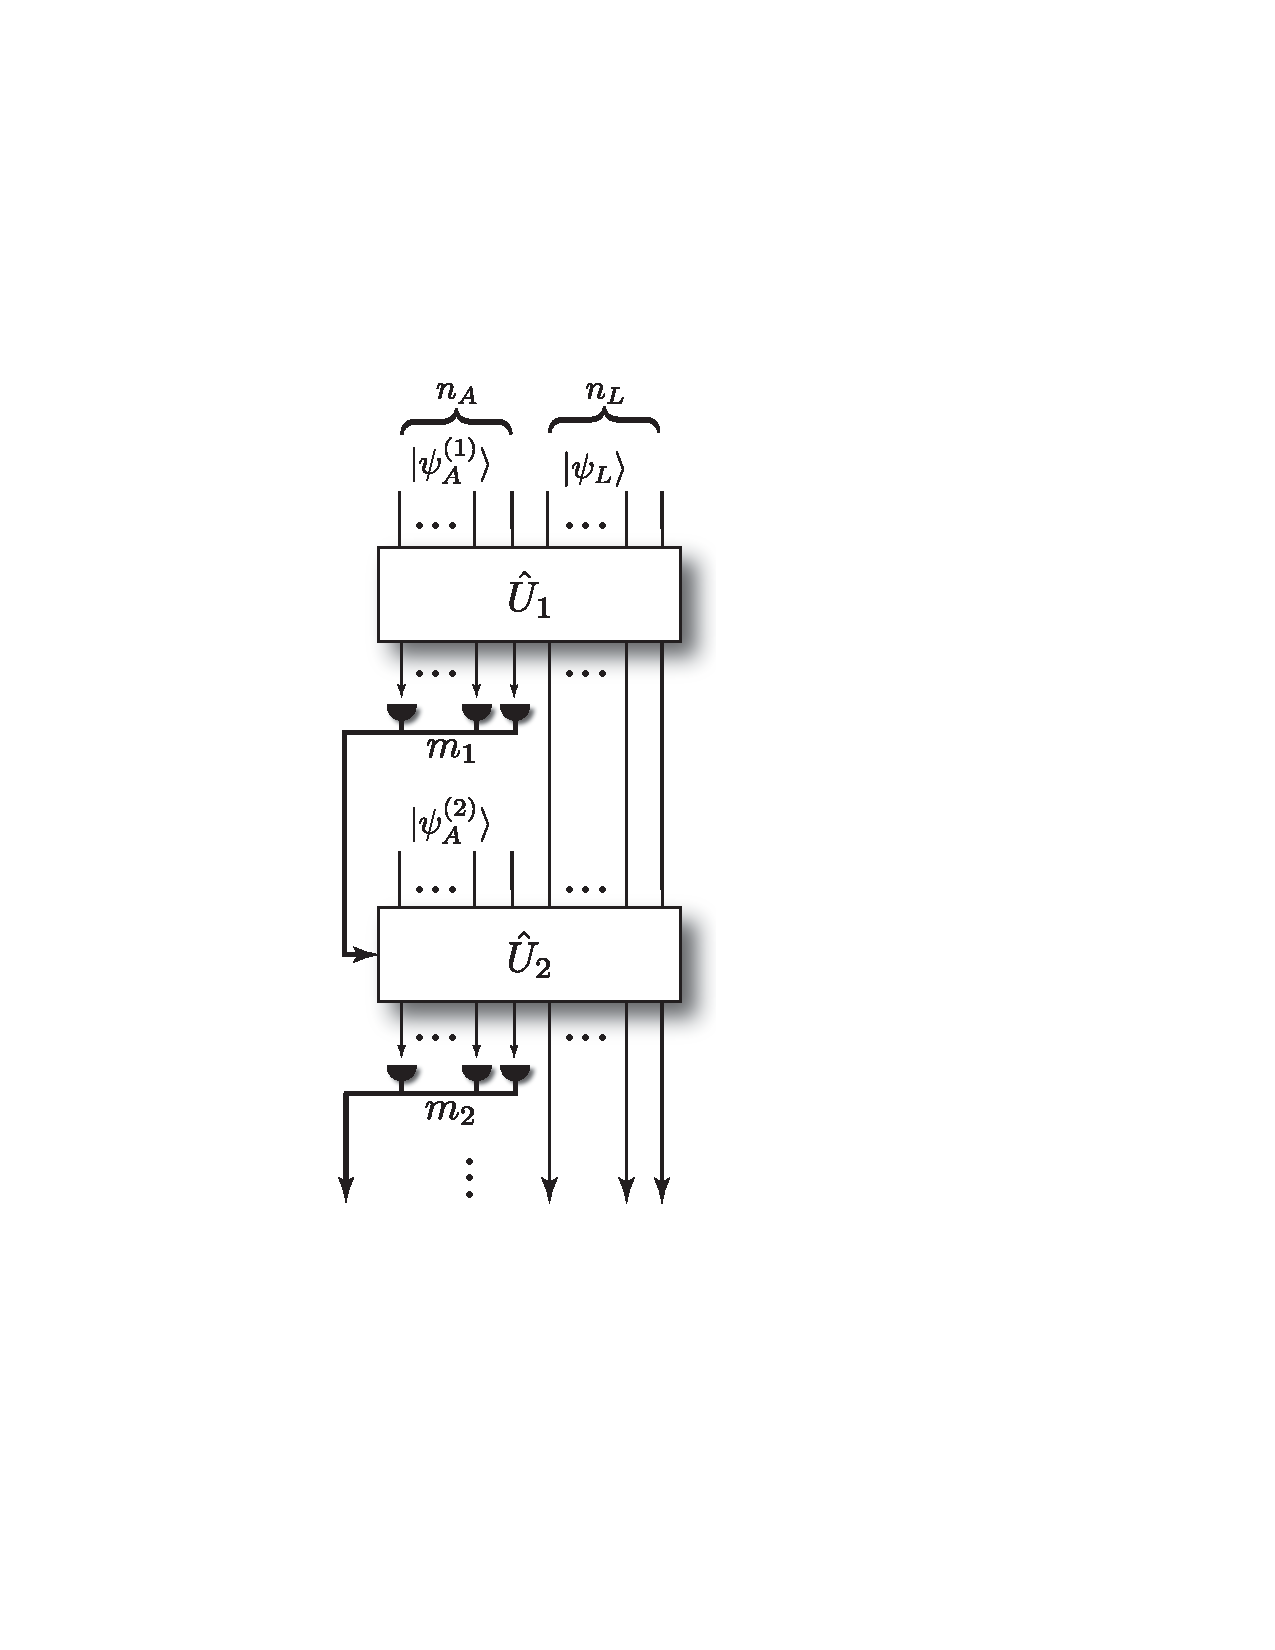
\includegraphics[width=0.5\columnwidth]{KLM}
\caption{KLM architecture for universal LOQC. $n_L$ optical modes are associated with logical qubits in the state $\ket{\psi_L}$, with the remaining $n_A$ modes acting as ancillary states, $\ket{\psi_A}$. A round of passive linear optics is applied, $\hat{U}_1$. Then the ancillary modes are measured, yielding some set of measurement outcomes $m_1$. These are classically processed to determine what the next round of passive linear optics, $\hat{U}_2$, ought to be. This repeats some polynomial number of times, from which an arbitrary quantum computation can be implemented. The \textsc{BosonSampling} and quantum walk models are equivalent to taking just the first stage of this protocol: one round of input state, passive linear optics, and measurement.} \label{fig:KLM_protocol}\index{Knill-Laflamme-Milburn (KLM)}
\end{figure}

Evolution via linear optics implements transformations of the form of Eq.~(\ref{eq:LO_unitary_map}), and may be implemented using the experimental architectures described in Sec.~\ref{sec:LO_ev_archs} and Fig.~\ref{fig:LO_archs}.

The measurements are implemented simply by number-resolved photo-detectors, implementing measurement projectors of the form \mbox{$\hat\Pi_n=\ket{n}\bra{n}$}, for the measurement outcome of $n$ photons (Sec.~\ref{sec:photo_detection}).

Since the original presentation of a universal LOQC gate set by KLM, numerous alternate implementations have been presented and experimentally demonstrated, with various pros and cons \cite{bib:Ralph01, bib:Pittman01, bib:Ralph02, bib:Knill02, bib:Pittman03, bib:MorYoran06}.

Although the original KLM scheme is universal, resource usage can be reduced by orders of magnitude by combining concepts from LOQC with the cluster state formalism (Sec.~\ref{sec:CSQC}) or related concepts \cite{bib:YoranReznik03, bib:Nielsen04, bib:BrowneRudolph05, bib:GilchristHayes05, bib:Lim05, bib:LimBarrett05}. Specifically, instead of using our non-deterministic KLM CZ gates within the circuit model formalism, they could be employed for the preparation of cluster states. Cluster state preparation using non-deterministic entangling gates is discussed in more detail in Sec.~\ref{sec:module}.

Significant progress is being made on reconfigurable, integrated LOQC devices \cite{bib:UniversalLOOBrien}, but switching times remain orders of magnitude slower than that required for fast-feedforward. The resource overhead associated with overcoming the non-determinism of entangling gates is substantial in the original KLM proposal. But despite being improved upon by cluster state approaches, resource scaling remains daunting. It therefore seems most likely that certain elements from LOQC might be combined into hybrid architectures, to be discussed in detail in Sec.~\ref{sec:hybrid}.

%
% Cluster State Linear Optics
%

\subsection{Cluster state linear optics} \label{sec:CS_LO} \index{Cluster states}

Sec.~\ref{sec:opt_stab}
Sec.~\ref{sec:module}

\comment{To do!}

%
% Fusion Gates
%

\subsubsection{Fusion gates} \index{Cluster state fusion gates}

As introduced in Sec.~\ref{sec:CSQC}, a cluster state may be defined by the action of CZ gates upon a graph of qubits initialised into the $\ket{+}$ state. As we saw in the previous section, implementing these CZ gates is troublesome using linear optics, as it is non-deterministic and carries the burden of a large resource overhead. Nonetheless, it was shown early on \cite{NielsenOptCS} that by combining non-deterministic CZ gates with the cluster state formalism yields LOQC protocols far more efficient than the original KLM protocol for LOQC.

It was then noted \cite{BrowneRudolph} that CZ gates aren't required at all for the preparation of optical cluster states. Instead, parity measurements (Sec.~\ref{sec:bell_proj}) operating in a rotated basis may be used to fuse smaller cluster states into larger ones, albeit acting destructively on two of the qubits, and also being non-deterministic, with a success probability of $1/2$. These gates have become known as \textit{fusion gates}, of which there are two types:
\begin{itemize}
	\item Type-I: destroy only a single photon, but require efficient number-resolved detection.
	\item Type-II: destroy two photons, but only require on/off detectors.
\end{itemize}
Both types of gates have several highly favourable characteristics:
\begin{itemize}
	\item Only HOM stability is required (Sec.~\ref{sec:opt_stab}). At no stage in the cluster state preparation procedure is any interferometric (i.e wavelength-scale) stability required.
	\item Gate failure is heralded by measurement of the wrong photon-number.
	\item Gate failure measures the respective qubits in the computational basis, thereby simply removing those qubits from the cluster state graph, whilst preserving the remainder of the state.
\end{itemize}

\comment{To do!}

%
% Fusion Strategies
%

\subsubsection{Fusion strategies} \index{Cluster state fusion strategies}

Despite their non-determinism, numerous authors have examined approaches for efficiently preparing arbitrarily large cluster states using these destructive, non-deterministic gates.

\comment{To do!}

%
% Advantages
%

\subsubsection{Advantages} \index{Cluster state advantages}

\comment{To do!}

%
% Weak Cross-Kerr Non-Linearities
%

\subsection{Weak cross-Kerr non-linearities} \index{Weak cross-Kerr non-linearity quantum computation}

More recently, as an alternative to using post-selection to simulate strong optical non-linearities, it was shown that by introducing strong coherent states, the strength of a cross-Kerr optical non-linearity can be effectively amplified, allowing even very weak non-linearities to be employed for deterministic entangling gate operations \cite{bib:Munro05}. However, such schemes are particularly sensitive to loss, with sensitivity increasing with the coherent amplitudes in the system, creating a direct tradeoff between effective non-linear interaction strength and susceptibility to loss.

\comment{To do! Bill Munro perhaps?}
\index{Quantum bus (Qubus)}

%
% Passive Linear Optics
%

\subsection{Passive linear optics} \label{sec:passive_LO} \index{Passive linear optics quantum computation}

While the KLM protocol (and subsequent improvements, e.g using cluster states) are universal for quantum computing, some of the key technological requirements are very challenging, and unlikely to be achieved in the short-term. However, simplified yet non-universal models for optical quantum computing can abandon some of the more challenging requirements, nonetheless implementing a restricted set of post-classical quantum computations. In particular, we consider protocols requiring only photon-number state preparation, passive linear optics evolution [as per Eq.~(\ref{eq:LO_unitary_map})], and photo-detection.

Optically, the two main contenders for this are multi-photon quantum walks \cite{bib:Aharonov93, bib:Aharonov01, bib:Kempe03, bib:Childs09, bib:Salvador12, bib:RohdeMultiWalk11} and \textsc{BosonSampling} \cite{bib:AaronsonArkhipov10, bib:RohdeIntroBS15}, both closely related in that they require only passive linear optics and single-photon states, whilst mitigating the need for active switching, quantum memory and dynamic fast-feedforward. Since, evidence has been presented that similar passive linear optics protocols may implement computationally hard problems using states of light other than photon-number states \cite{bib:RandBS, bib:RohdePhotAdd15, bib:RohdeDisp15, bib:RohdeCat15}.

These protocols involve nothing more than evolving multiple single-photon states through beamsplitter networks and measuring the output photo-statistics. This is equivalent to just taking the first stage of the KLM protocol shown in Fig.~\ref{fig:KLM_protocol}.

Both quantum walks and \textsc{BosonSampling} have been subject to extensive experimental investigation in recent years \cite{bib:PeruzzoQW, bib:Broome10, bib:Schreiber11b, bib:Owens11, bib:RohdeQWExp12, bib:Broome2012, bib:RohdeQWExp12, bib:Spring2, bib:Crespi3, bib:Tillmann4}.

Because these models are entirely passive, they can be made cloud-based very trivially: Alice prepares her permutation of single photons as the input state, sends it to Bob over the quantum network, who applies the passive operations before returning the state to Alice. In this case, no intermediate client/server interaction is required. Alternately, she could classically communicate a bit-string to Bob indicating the input photon-number configuration, in case she is unable to prepare it herself.

The \textsc{BosonSampling} and quantum walk models are based on single-photon encoding. However, passive linear optics could also be applied to other states of light. In particular, passive linear optics acting upon multi-mode coherent states implements the \textit{classical} computation of matrix multiplication.

%
% Boson-Sampling
%

\subsubsection{{\sc BosonSampling}} \label{sec:BS} \index{Boson-sampling}

\textsc{BosonSampling} is the problem of sampling the output photon-number statistics of a linear optics interferometer fed with single-photon inputs. While not universal for quantum computing (in fact no one has any idea what to use it for at all!), there is strong evidence that it is a classically hard problem \cite{bib:AaronsonArkhipov10, bib:RohdeIntroBS15}.

The computational hardness of \textsc{BosonSampling} relates to the fact that the amplitudes in the output superpositions are proportional to matrix permanents, which are known to be \#\textbf{P}-hard\index{\textbf{\#P} \& \textbf{\#P}-complete} in general. This is believed to be a classically hard complexity class, even harder than \textbf{NP}-complete\index{\textbf{NP} \& \textbf{NP}-complete} in the complexity hierarchy, requiring exponential classical time to evaluate (see Fig.~\ref{fig:complexity_classes} for the believed complexity relationships). This yields computationally complex sampling problems.

%
% The Boson-Sampling Model
%

\paragraph{The {\sc BosonSampling} model} \index{Boson-sampling model}

For an $m$-mode interferometer, and input state,
\begin{align}
\ket\psi_\text{in} = \ket{T_1,\dots,T_m},
\end{align}
where there are $T_i$ photons in the $i$th input mode, the output superposition takes the form,
\begin{align}
\ket\psi_\text{out} = \sum_S \gamma_{S,T} \ket{S_1,\dots,S_m},
\end{align}
where $S$ sums over all possible photon-number configurations at the output, of which there are,
\begin{align}
|S| = \binom{n+m-1}{n},
\end{align}
where there are $n$ photons in total in $m$ modes. It is assumed that,
\begin{align}
m=O(n^2),
\end{align}
which, for large $m$, puts us into the anti-bunched (i.e binary photon-number) regime with high probability\footnote{That is, we are unlikely to observe more than a single photon in any given output mode, placing us into a binary photo-detection regime. This condition has become known as the `bosonic birthday paradox'.}, rendering non-number-resolved photo-detectors sufficient for physical implementation. However, this `no-collision' subspace remains exponentially large,
\begin{align}
|S_\text{no-collision}| = \binom{m}{n}.
\end{align}

The amplitudes $\gamma_{S,T}$ are given by,\index{Boson-sampling configuration amplitudes}
\begin{align}
	\gamma_{S,T} = \frac{\text{Per}(U_{S,T})}{\sqrt{S_1!\dots S_m! T_1!\dots T_m!}},
\end{align}
and the associated configuration probabilities by\index{Boson-sampling configuration probabilities},
\begin{align}
	P_{S,T} &= |\gamma_{S,T}|^2 \nonumber \\
	&= \frac{|\text{Per}(U_{S,T})|^2}{S_1!\dots S_m! T_1!\dots T_m!}
\end{align}
where $\text{Per}(\cdot)$ denotes the matrix permanent, and $U_{S,T}$ is a sub-matrix of $U$ -- the transfer matrix\index{Transfer matrix} associated with the particular input-to-output sample configuration -- obtained by taking $S_i$ copies of the $i$th row, and $T_j$ copies of the $j$th column of the linear optics unitary matrix $U$. For the purposes of the original complexity proof, the unitary is chosen randomly from the Haar-measure\footnote{The Haar-measure generalises the notion of a uniform distribution to higher-dimensional topologies than the real numbers, in this instance to the $\text{SU}(n)$ group.}\index{Haar measure}, although it remains an open question as to what is the full class of unitaries that yield computationally hard problems.

The computational problem is simply to sample this probability distribution $P_{S,T}$, which the linear optics network can implement efficiently, but it is believed a classical computer cannot. The full model is shown in Fig.~\ref{fig:bs_model}.

\begin{figure}[!htb]
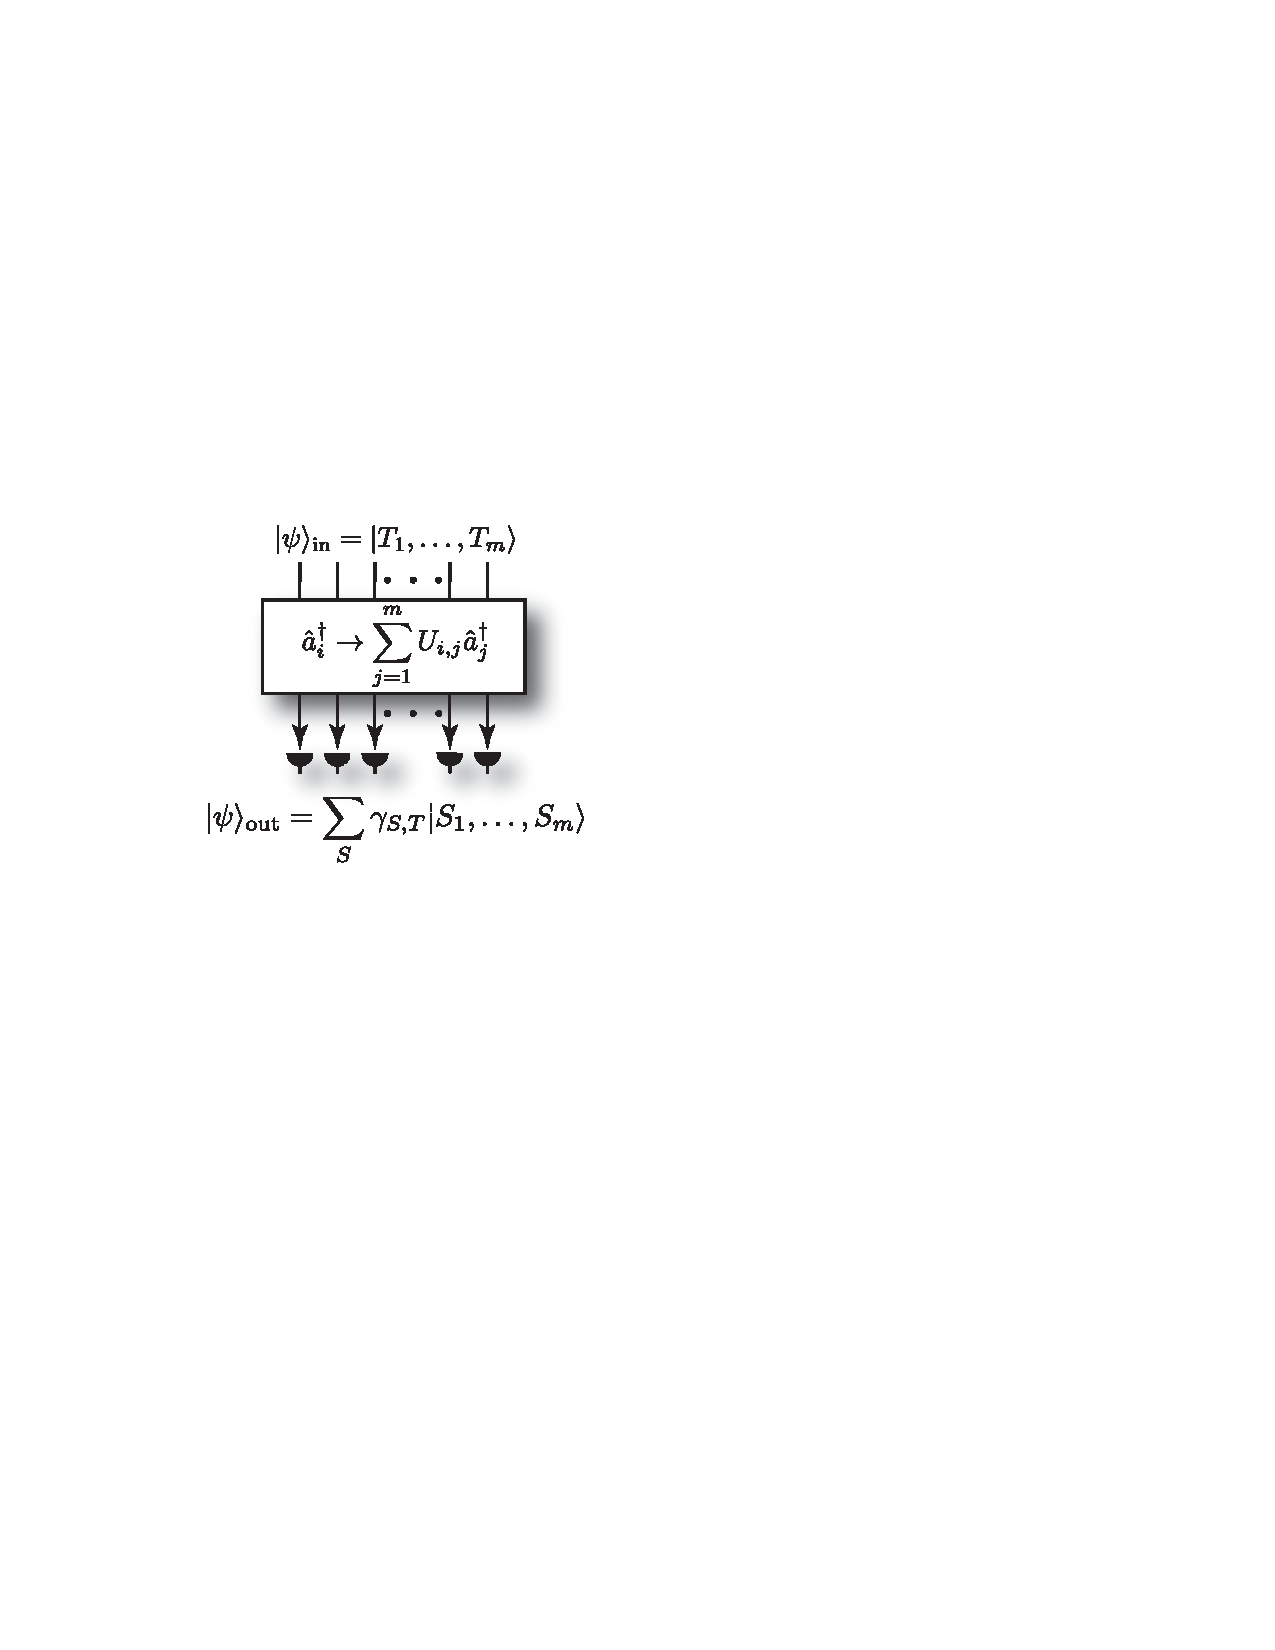
\includegraphics[width=0.7\columnwidth]{bs_model}
\caption{The \textsc{BosonSampling} model for non-universal linear optics quantum computing. $S$ (output) and $T$ (input) are represented in the photon-number basis. After application of the Haar-random linear optics unitary to the input multi-mode Fock state, the output superposition is sampled with coincidence photo-detection.} \label{fig:bs_model}
\end{figure}

For comparison, the equivalent classical protocol using distinguishable photons that evolve independently through the network would be described by,
\begin{align}
	P_{S,T} = \frac{\text{Per}(|U_{S,T}|^2)}{S_1!\dots S_m! T_1!\dots T_m!},
\end{align}
which yields a classically efficient sampling problem. Thus, for {\sc BosonSampling} the permanents are of complex-valued matrices, whereas for the equivalent classical problem the permanents are of positive real-valued matrices.

Very importantly, note that {\sc BosonSampling} does \textit{not} let us efficiently \textit{calculate} matrix permanents. Rather, it samples across a distribution of an exponential number of permanents. This is because, for an exponentially large sample space, with only a polynomial number of measurement trials, we are unlikely to gain more than binary accuracy about individual amplitudes, which is insufficient for determining any particular permanent. It appears that God knows how to efficiently solve matrix permanents, but conspires against us such that we remain ignorant of them. --- \textit{Deus magnus est.}

The size of a boson-sampler required to exhibit post-classicality is under active debate, as has undergone much historical revision \cite{RohdeRalph}. But some recent estimates suggest that as many as 50 photons in 2,500 modes might be a rough guide for such a threshold \cite{NoSupBS_Montanaro}. Needless to say, this is already an extremely challenging technological goal, suggesting that although the {\sc BosonSampling} problem is far simpler than universal LOQC, it is far from simple.

\textsc{BosonSampling} in the presence of various error models, such as loss, source non-determinism and mode-mismatch, has been extensively investigated \cite{bib:RohdeErrBS12, bib:RohdeSPDC13, bib:ScottLost16, bib:RohdeArbSpec15, bib:RandBS}. 

%
% Multiplexed Boson-Sampling
%

\paragraph{Multiplexed {\sc BosonSampling}} \index{Multiplexed boson-sampling}

As discussed in Sec.~\ref{sec:single_phot_src}, SPDC is the most common present-day implementation of single-photon sources. However, despite their ready availability, they suffer from non-determinism, with single-photon heralding probability given by Eq.~(\ref{eq:SPDC_p_prep}). To improve upon this, multiplexed sources can be employed \cite{bib:RohdeSPDC13}, improving effective single-photon preparation probabilities asymptotically to unity, as given by Eq.~(\ref{eq:SPDC_multiplex}).

However, rather than employing a multiplexed SPDC source in place of each of the required $n$ single-photons, we can instead employ a larger multiplexer that routes \mbox{$N\gg n$} sources to $n$ modes, which is far more efficient than $n$ independent multiplexed single-photon sources.

The model is shown in Fig.~\ref{fig:multiplexed_bs}. We begin by operating $N$ SPDC sources in parallel. Clearly if $N$ is sufficiently large with respect to $n$, it becomes asymptotically certain that at least $n$ photons will be heralded. When this occurs, the successfully prepared $n$ photons -- in whatever configuration they happen to occur -- are routed to the first $n$ modes of the {\sc BosonSampling} interferometer $\hat{U}$ by the multiplexer (which is classically controlled by the SPDC heralding outcomes), and the protocol proceeds as usual.

\begin{figure}[!htb]
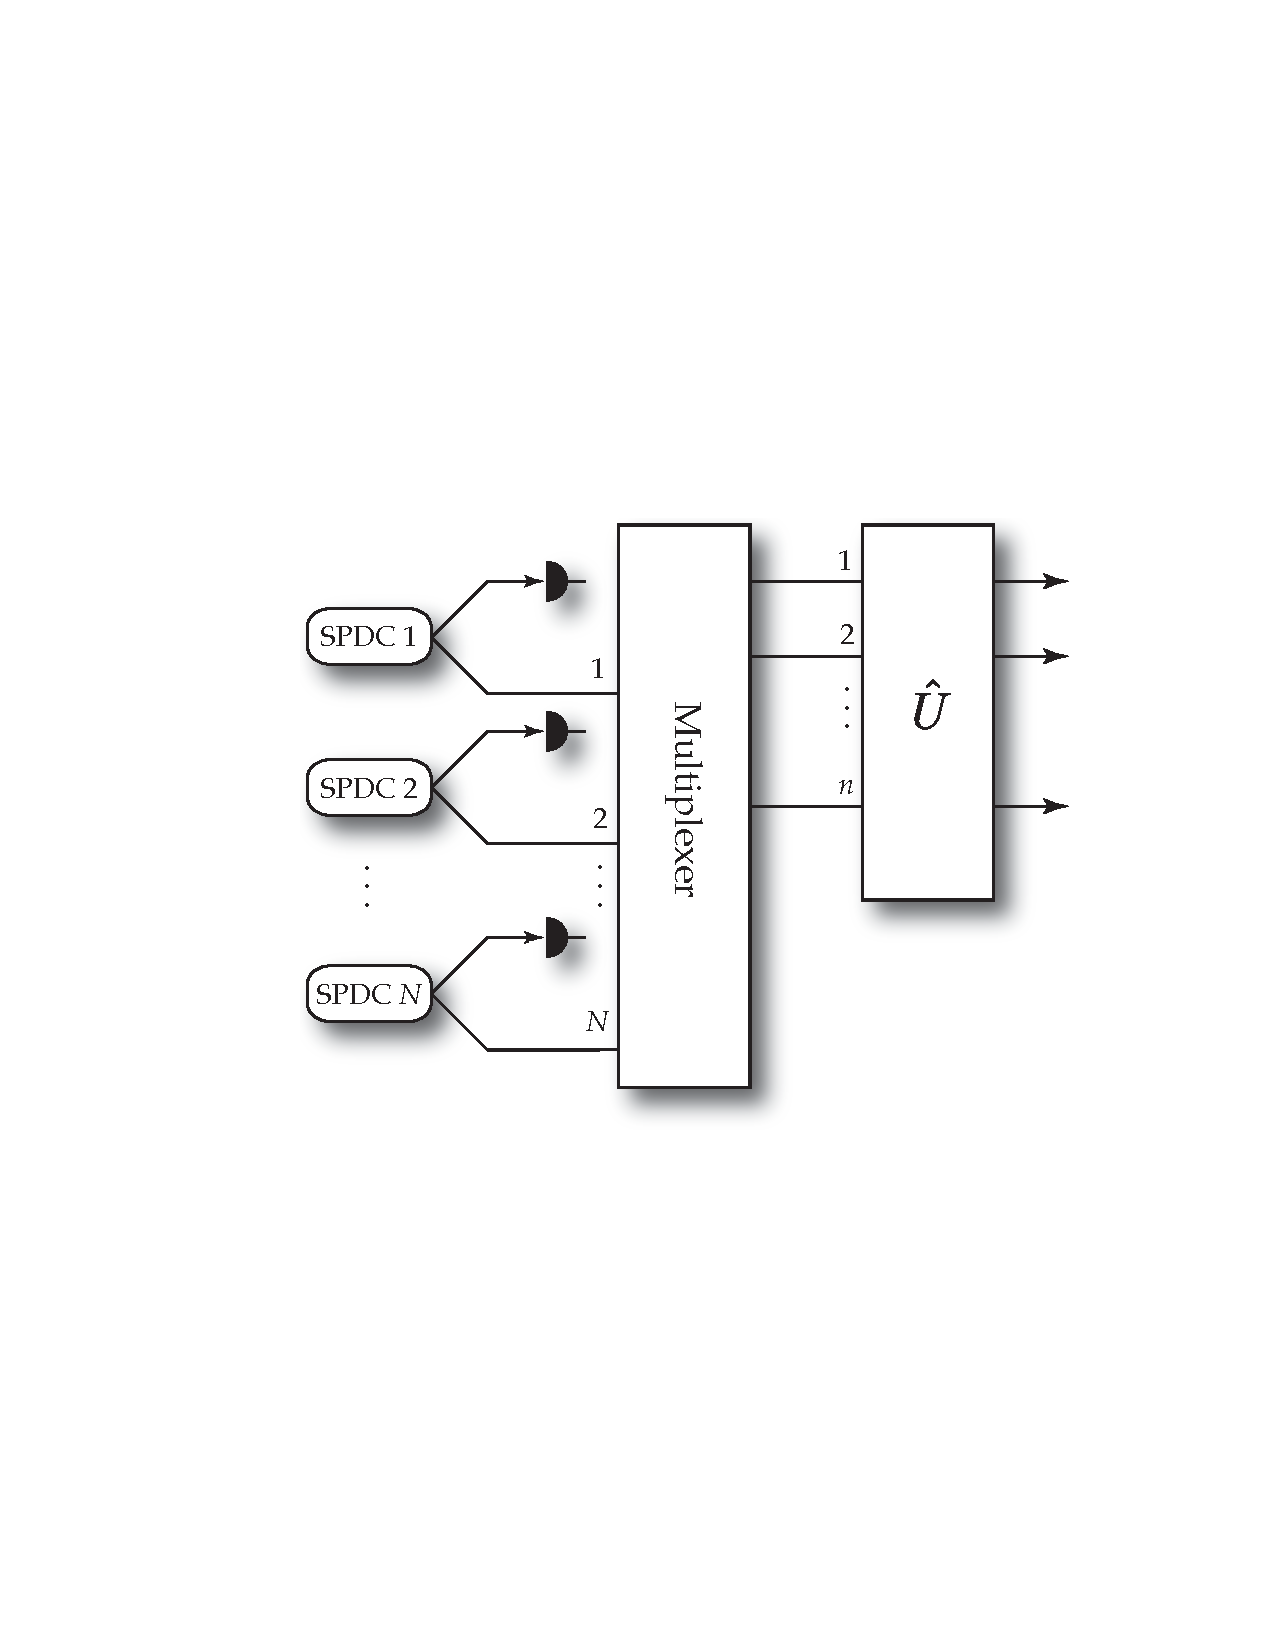
\includegraphics[width=\columnwidth]{multiplexed_boson_sampling}
\caption{Model for multiplexed {\sc BosonSampling}. We operate \mbox{$N\gg n$} SPDC sources in parallel, which are multiplexed to the first $n$ modes of the interferometer $\hat{U}$. With sufficiently large $N$ it becomes asymptotically certain that at least $n$ single-photons will be heralded, thereby successfully preparing the desired {\sc BosonSampling} input state.} \label{fig:multiplexed_bs}\index{Multiplexed boson-sampling}
\end{figure}

Specifically, the probability of at least $n$ successful single-photon heralding events occurring is,
\begin{align}
P_{\geq n} = \sum_{i=n}^\infty \binom{N}{i} 	{P_\text{herald}}^i (1-P_\text{herald})^{N-i},
\end{align}
where,
\begin{align}
	P_\text{herald} = \chi^2(1-\chi^2),
\end{align}
is the probability of a single SPDC source heralding the preparation of a single-photon. This quantity asymptotes to unity for \mbox{$N\gg n$}, as shown in Fig.~\ref{fig:multiplex_bs_res}.

\begin{figure}[!htb]
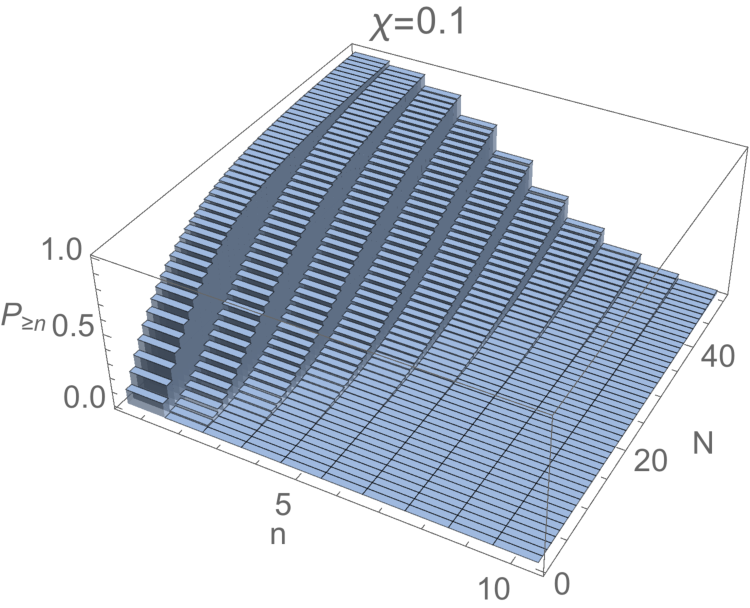
\includegraphics[width=0.95\columnwidth]{multiplex_bs}
\caption{Probability of successfully preparing at least $n$ photons for {\sc BosonSampling} from a multiplexed source comprising a bank of $N$ SPDC sources in parallel. For sufficiently large $N$, we prepare the desired $n$ photons with probability asymptoting to unity.} \label{fig:multiplex_bs_res}\index{Multiplexed boson-sampling}
\end{figure}

However, although this procedure works in-principle, it comes at the expense of a large number of sources, $N$, and more challengingly, fast-feedforward. Keep in mind that if we were able to perform complex fast-feedforward, we might be able to do much more (and far more interesting things) than just {\sc BosonSampling} in the first place!

%
% Scattershot Boson-Sampling
%

\paragraph{Scattershot {\sc BosonSampling}} \index{Scattershot boson-sampling}

A variation on SPDC-based {\sc BosonSampling}, known as `scattershot'\index{Scattershot boson-sampling} {\sc BosonSampling}, has been presented \cite{bib:RandBS}, which obviates the difficultly of fast multiplexing in the approach described previously. Here, rather than inputting an SPDC source into the first $n$ of the $m$ modes, we input a source into \textit{every} mode, i.e $m$ sources in total. We then accept all events with $n$ heralding successes in total, irrespective of the configuration in which they occur. This has the effect of implementing $n$-photon {\sc BosonSampling} with an additional layer of randomisation on the input modes (i.e a randomisation in the input configuration, $T$, which is ordinarily fixed). However, since the algorithm is already randomised, this additional layer of randomisation does not undermine the complexity proofs, which hold as is. The scattershot model is shown in Fig.~\ref{fig:scattershot_model}.

\begin{figure}[!htb]
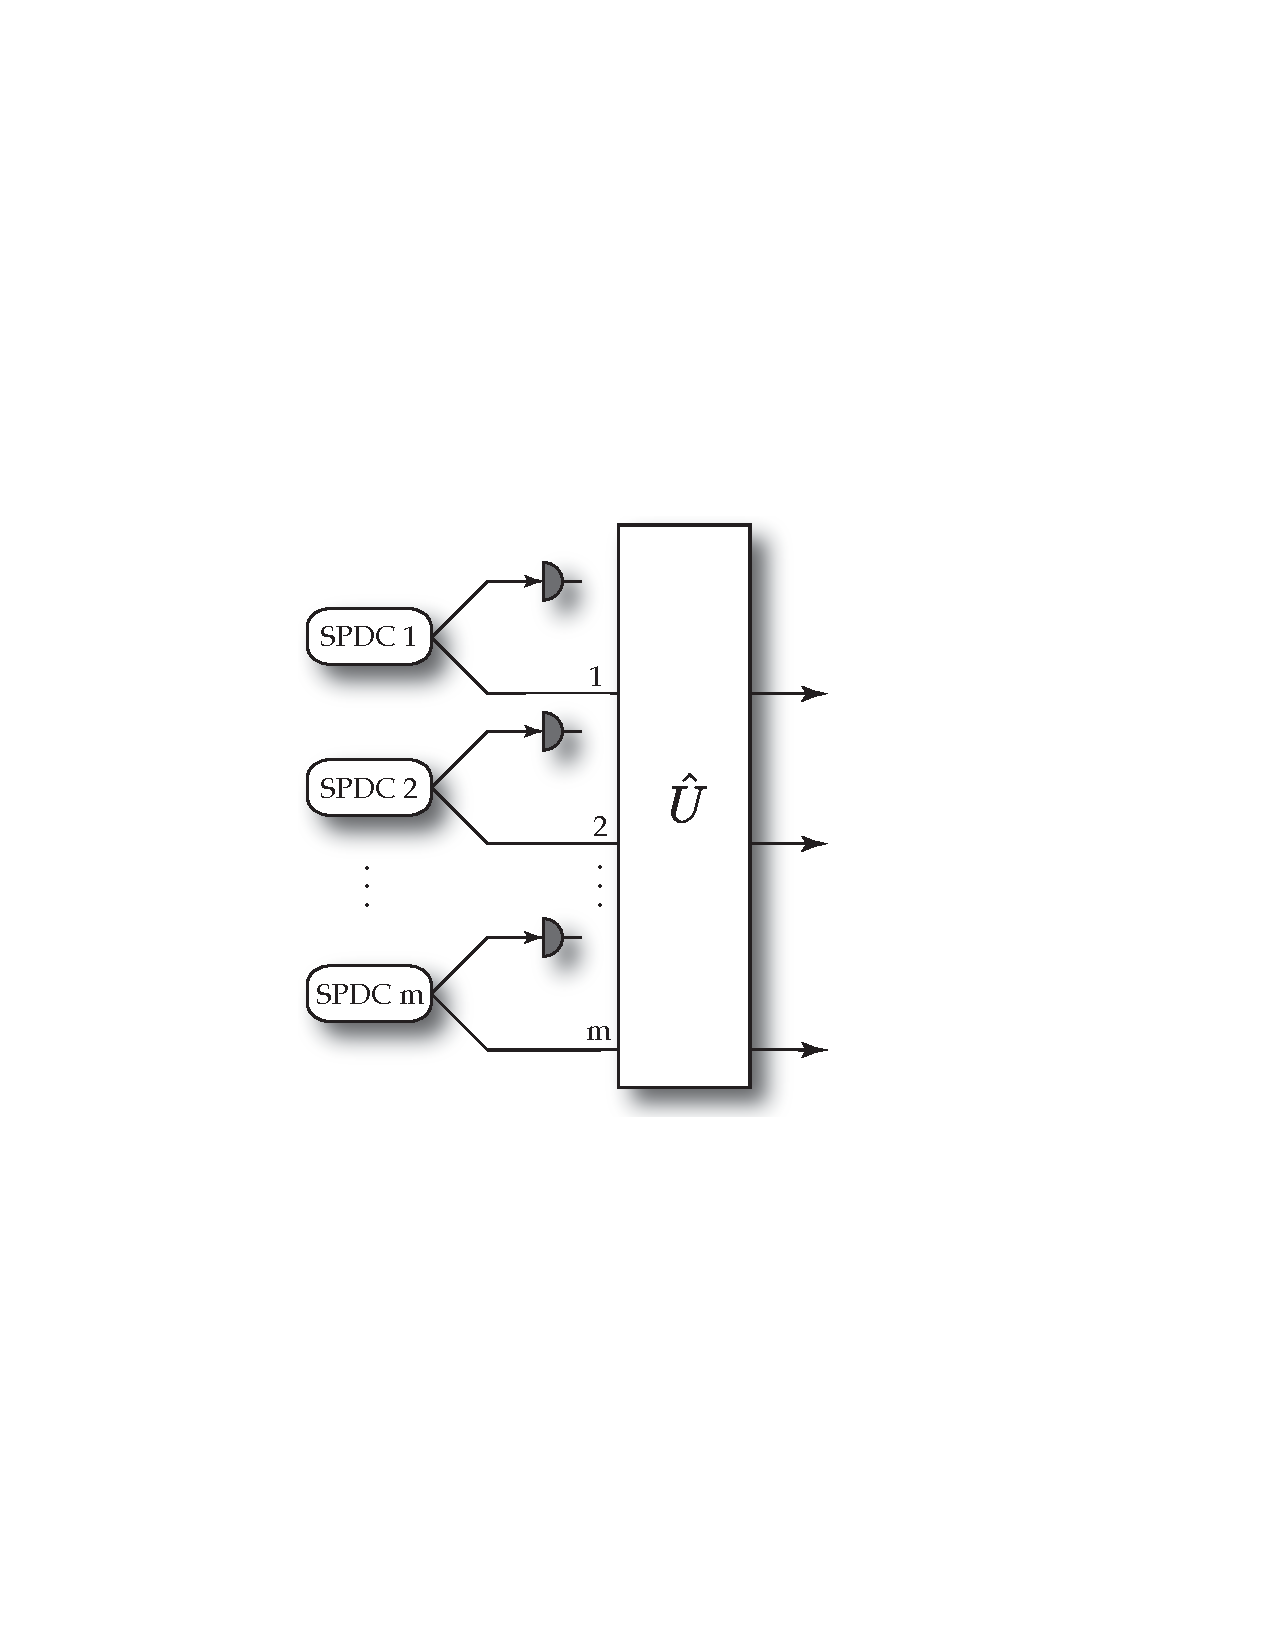
\includegraphics[width=0.7\columnwidth]{scattershot_model}
\caption{Model for `scattershot' {\sc BosonSampling}. An SPDC source is inputted into all $m$ input modes. We post-select upon detecting a total of $n$ photons in the heralding modes, irrespective of their configuration, yielding an $n$-photon instance of {\sc BosonSampling} with randomised input configuration. Unlike multiplexed architectures, the scheme remains entirely passive, without requiring adaptive fast-feedforward.} \label{fig:scattershot_model}
\end{figure}

By keeping all configurations of $n$ photons, rather than just the \mbox{$\ket{T}=\ket{1}^{\otimes n} \ket{0}^{\otimes (m-n)}$} case, we effectively boost the $n$-photon heralding probability from,
\begin{align}
	P_n = \chi^{2n}(1-\chi^2)^n,	
\end{align}
to,
\begin{align}
	P_n = \binom{n^2}{n}\chi^{2n}(1-\chi^2)^{n^2},	
\end{align}
exhibiting a binomial enhancement in $n$-photon events, yielding a significant improvement in count-rates. For a given desired photon-number $n$, choosing the value for the squeezing parameter, $\chi$, which maximises $P_n$, we obtain the optimised success probability,
\begin{align}
	P_n^{(\text{opt})} \approx \frac{1}{e\sqrt{2\pi(n-1)}},
\end{align}
which exhibits only polynomial scaling against photon-number $n$, and is therefore scalable. This is shown in Fig.~\ref{fig:scattershot_probs}. This is in stark contrast to conventional {\sc BosonSampling}, where the success probability decays exponentially with photon-number, and is therefore inefficient. Importantly, unlike the multiplexed approach, this efficiency improvement does not require any active elements, remaining in the true spirit of {\sc BosonSampling}.

\begin{figure}[!htb]
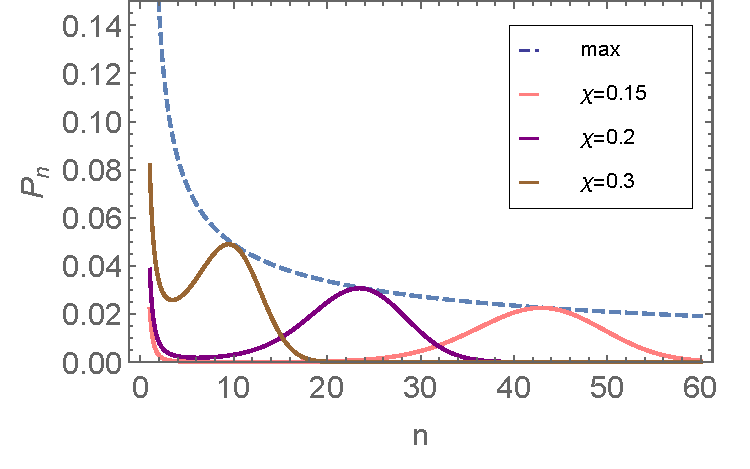
\includegraphics[width=\columnwidth]{scattershot_probs}
\caption{Probability of successfully implementing an instance of $n$-photon {\sc BosonSampling} using the scattershot technique, whereby all input modes are fed with an SPDC source, and all $n$-photon heralding events are accepted, irrespective of their configuration.} \label{fig:scattershot_probs}
\end{figure}

%
% Other Linear Optics Sampling Problems
%

\subsubsection{Other linear optics sampling problems} \label{sec:other_LO_samp_probs} \index{Linear optics sampling problems}

In addition to photonic \textsc{BosonSampling}, several authors have presented strong evidence that other classes of quantum states of light exist, which yield computationally complex sampling problems under the action of linear optics. Most notably, such evidence has been provided for the following:
\begin{itemize}
\item \cite{bib:RandBS} considered two-mode squeezed vacuum (or SPDC) states, a type of Gaussian state with strictly positive Wigner function. This is the same as the scattershot model presented in Sec.~\ref{sec:BS}.\index{Two-mode squeezed vacuum states}\index{Gaussian states}
	\begin{align}
		\ket\psi_\text{in} = \sqrt{1-\chi^2}\sum_{n=0}^\infty \chi^n\ket{n,n}.
	\end{align}
\item \cite{bib:RohdeDisp15} considered photon-added coherent states and displaced single-photon states.\index{Photon-added coherent states}\index{Displaced single-photon states}
	\begin{align}
		\ket\psi_\text{in} &\propto \hat{a}^\dag\ket\alpha,\\
		\ket\psi_\text{in} &\propto \hat{D}(\alpha)\ket{1}.
	\end{align}
\item \cite{bib:RohdePhotAdd15} considered photon-added or -subtracted squeezed vacuum states.\index{Photon-added squeezed vacuum states}\index{Photon-subtracted squeezed vacuum states}
	\begin{align}
		\ket\psi_\text{in} &\propto \hat{a}^\dag\hat{S}(\chi)\ket{0},\\
		\ket\psi_\text{in} &\propto \hat{a}\hat{S}(\chi)\ket{0}.
	\end{align}
\item \cite{bib:RohdeCat15} considered `cat' states -- superpositions of coherent states.\index{Cat states}
	\begin{align}
		\ket\psi_\text{in} \propto \ket\alpha \pm \ket{-\alpha}.
	\end{align}
\end{itemize}

Preparation of all of these classes of quantum states of light present their own technological challenges, some very daunting, and all much harder to prepare than single-photons. Thus, the ability to outsource their preparation would be a useful application for the quantum cloud.

On the other hand, some classes of optical states are known to be efficiently classically simulable under linear optics evolution and photo-detection. This includes coherent states, thermal states, or any state with strictly positive $P$-function\footnote{A strictly positive $P$-function implies that the state can be considered a purely classical mixture of coherent states (each of which are classically efficient to simulate), according to some probability distribution.} (Sec.~\ref{sec:exotic}) \cite{bib:SalehQOCCC15, bib:SalehEffSim16}. Furthermore, Gaussian states evolved via linear optics and measured using Gaussian measurements have been shown to be computationally easy to simulate \cite{bib:Bartlett02, bib:Bartlett02b}.

\comment{Cite Saleh/Carlton paper on most optical states generating entanglement. Is it exponential entanglement? If so, is this a necessary but not sufficient condition for computational complexity.}

%
% Quantum Walks
%

\subsubsection{Quantum walks} \label{sec:QW} \index{Quantum walks}

Photonic quantum walks (QWs) are the other main contender for implementing restricted quantum computation, without requiring the full spectrum of challenging LOQC operations. The resource requirements are the same as for \textsc{BosonSampling}, the difference being that now instead of choosing a Haar-random unitary matrix for the interferometer, we choose one which encodes a graph. The photons are now referred to as `walkers', and they evolve by following edges within the graph, `hopping' between neighbouring vertices.

With only a single walker (photon), nothing computationally complex can occur in the system, since a single photon evolving under passive linear optics can be efficiently classically simulated\footnote{Note that the literature has described QW schemes, both discrete-time \cite{bib:Lovett10} and continuous-time \cite{bib:Childs09}, that are universal for quantum computation. However, such universal schemes require an exponential number of vertices in the underlying graph, which clearly does not lend itself to efficient optical representation.}. However, once multiple walkers are introduced we have a system with almost identical features to \textsc{BosonSampling}, differing only in the structure of the linear optics unitary.

There are two predominant varieties of quantum walks: discrete- \cite{qwDiscrete:aharanov} and continuous-time \cite{contTimeQW:childs}, which we will now introduce. Algorithms have been described for both the discrete- and continuous-time QW models.

%
% Continuous-Time Quantum Walks
%

\paragraph{Continuous-time quantum walks}\index{Continuous-time quantum walks}

In the continuous-time QW model, a Hamiltonian, $\hat{H}_\text{QW}$, encoding the (Hermitian) adjacency matrix of the QW's graph evolves the walker(s), generating a unitary evolution of the form,
\begin{align}\index{Quantum walk Hamiltonian}
\hat{U}_\text{QW}(t) = e^{-i\hat{H}_\text{QW}t},
\end{align}
where \mbox{$t\in \mathbb{R}_+$}.

This model lends itself readily to optical wave-guide\index{Waveguides} implementation, where evanescent coupling between neighbouring wave-guides is inherently a continuous-time process. Fig.~\ref{fig:LO_archs}(c) illustrates an example implementation of a linear optics, continuous-time quantum walk on a line in an integrated wave-guide device.

In the context of linear optics, the evolution is best described using the coupled oscillator Hamiltonian\index{Coupled oscillator Hamiltonian},
\begin{align}
	\hat{H}_\text{QW} = \sum_{i,j=1}^m c_{i,j} \hat{a}^\dag_i\hat{a}_j,
\end{align}
where $\hat{a}^\dag_i$ ($\hat{a}_i$) is the photonic creation (annihilation) operator for the $i$th of the $m$ modes, and the Hermitian matrix $c_{i,j}$ encodes the coupling strength between the $i$th and $j$th modes, which could correspond identically to the QW's graph adjacency matrix.

%
% Discrete-Time Quantum Walks
%

\paragraph{Discrete-time quantum walks}\index{Discrete-time quantum walks}

In the discrete-time QW model, each walker has access to an ancillary `coin' Hilbert space, which is used to record the direction of the walker through the graph. At each discrete time-step the coin is used to update the position (vertex) of the walker, before applying a unitary `coin' operator to the coin Hilbert space. The addition of the coin space is necessary to enable such quantum walks to reside on arbitrary graph topologies, whilst retaining unitarity in their evolution. 

We will briefly summarise the discrete-time QW model, as it most readily lends itself to linear optics implementation, and illustrate the parallels with \textsc{BosonSampling}. First, let us consider the standard simple example scenario of a single quantum walker, on a linear graph topology, using a Hadamard coin\index{Hadamard gate},
\begin{align}
\hat{C} = \frac{1}{\sqrt{2}}\begin{pmatrix}1 & 1 \\
1 & -1
\end{pmatrix},
\end{align}
which has been experimentally demonstrated using both bulk-optics \cite{bib:Broome10} and time-bin encoding \cite{bib:Schreiber10, bib:RohdeQWExp12}. The walker is defined by two Hilbert spaces: the position $x$, and the coin {$c=\pm 1$}, where $+1$ ($-1$) indicates that the walker is moving to the right (left). The basis states are then $\ket{x,c}$, and the state of the walker takes the form,
\begin{align}
\ket\psi = \sum_{x,c} \lambda_{x,c} \ket{x,c}.
\end{align}
The evolution of the walk is given by the coin and step operators,
\begin{align} \index{Coin operators}\index{Step operators}
\hat{C}\ket{x,\pm 1} &\to \frac{1}{\sqrt{2}}(\ket{x,+1}\pm \ket{x,-1}), \nonumber \\
\hat{S}\ket{x,c} &\to \ket{x+c,c}.
\end{align}
The Hadamard coin operator could be replaced with any arbitrary $\text{SU}(2)$ matrix. The total time-evolution of the walk is then given by,
\begin{align}
\ket{\psi(t)} = (\hat{S}\hat{C})^t\ket{\psi(0)},
\end{align}
where \mbox{$t\in\mathbb{Z}_+$}. Upon measurement, the probability of the walker being at position $x$ is simply given by summing the probabilities over the coins at a given position,
\begin{align}
P(x) = |\lambda_{x,-1}|^2 + |\lambda_{x,+1}|^2.
\end{align}

The single-walker walk on a linear graph is not of computational interest as it can be efficiently classically simulated. However, the formalism is easily logically generalised to multiple walkers on arbitrary graph topologies. We will illustrate this using the formalism of \cite{bib:RohdeMultiWalk11}, where \textit{walker operators}\index{Walker operators}, rather than walker basis states are evolved under time-evolution (i.e we operate in the Heisenberg picture rather than the Schr{\" o}dinger picture). In an optical context, walker operators are identically photonic creation operators. The walker operators are of the form $\hat{w}(x,c)^\dag$, where $x$ denotes the vertex number currently occupied by the walker, and $c$ denotes the previous vertex occupied by the walker. The single-walker basis states are then of the form $\hat{w}(x,c)^\dag\ket{0}$, where $\ket{0}$ is the vacuum state containing no excitations. Notice the parallels to the previous example of a linear walk, where the coin degree of freedom specifies the direction the walker is following, which effectively acts as memory of the previous position.

The coin and step operators now take the form,
\begin{align}
\hat{C}: \,\,\, &\hat{w}(x,c)^\dag \to \sum_{j\in n_x}A_{c,j}^{(x)} \hat{w}(x,j)^\dag, \nonumber \\
\hat{S}: \,\,\, &\hat{w}(x,j)^\dag \to \hat{w}(j,x)^\dag.
\end{align}
Here $n_x$ denotes the set of vertices neighbouring $x$. The coin operators $A^{(x)}$ are \mbox{$\text{SU}(|n_x|)$} unitary matrices representing the weights of edges within this neighbourhood. The step operator, on the other hand, is simply a permutation. A simple example is shown in Fig.~\ref{fig:QW_arbitrary_graph}.

\begin{figure}[!htb]
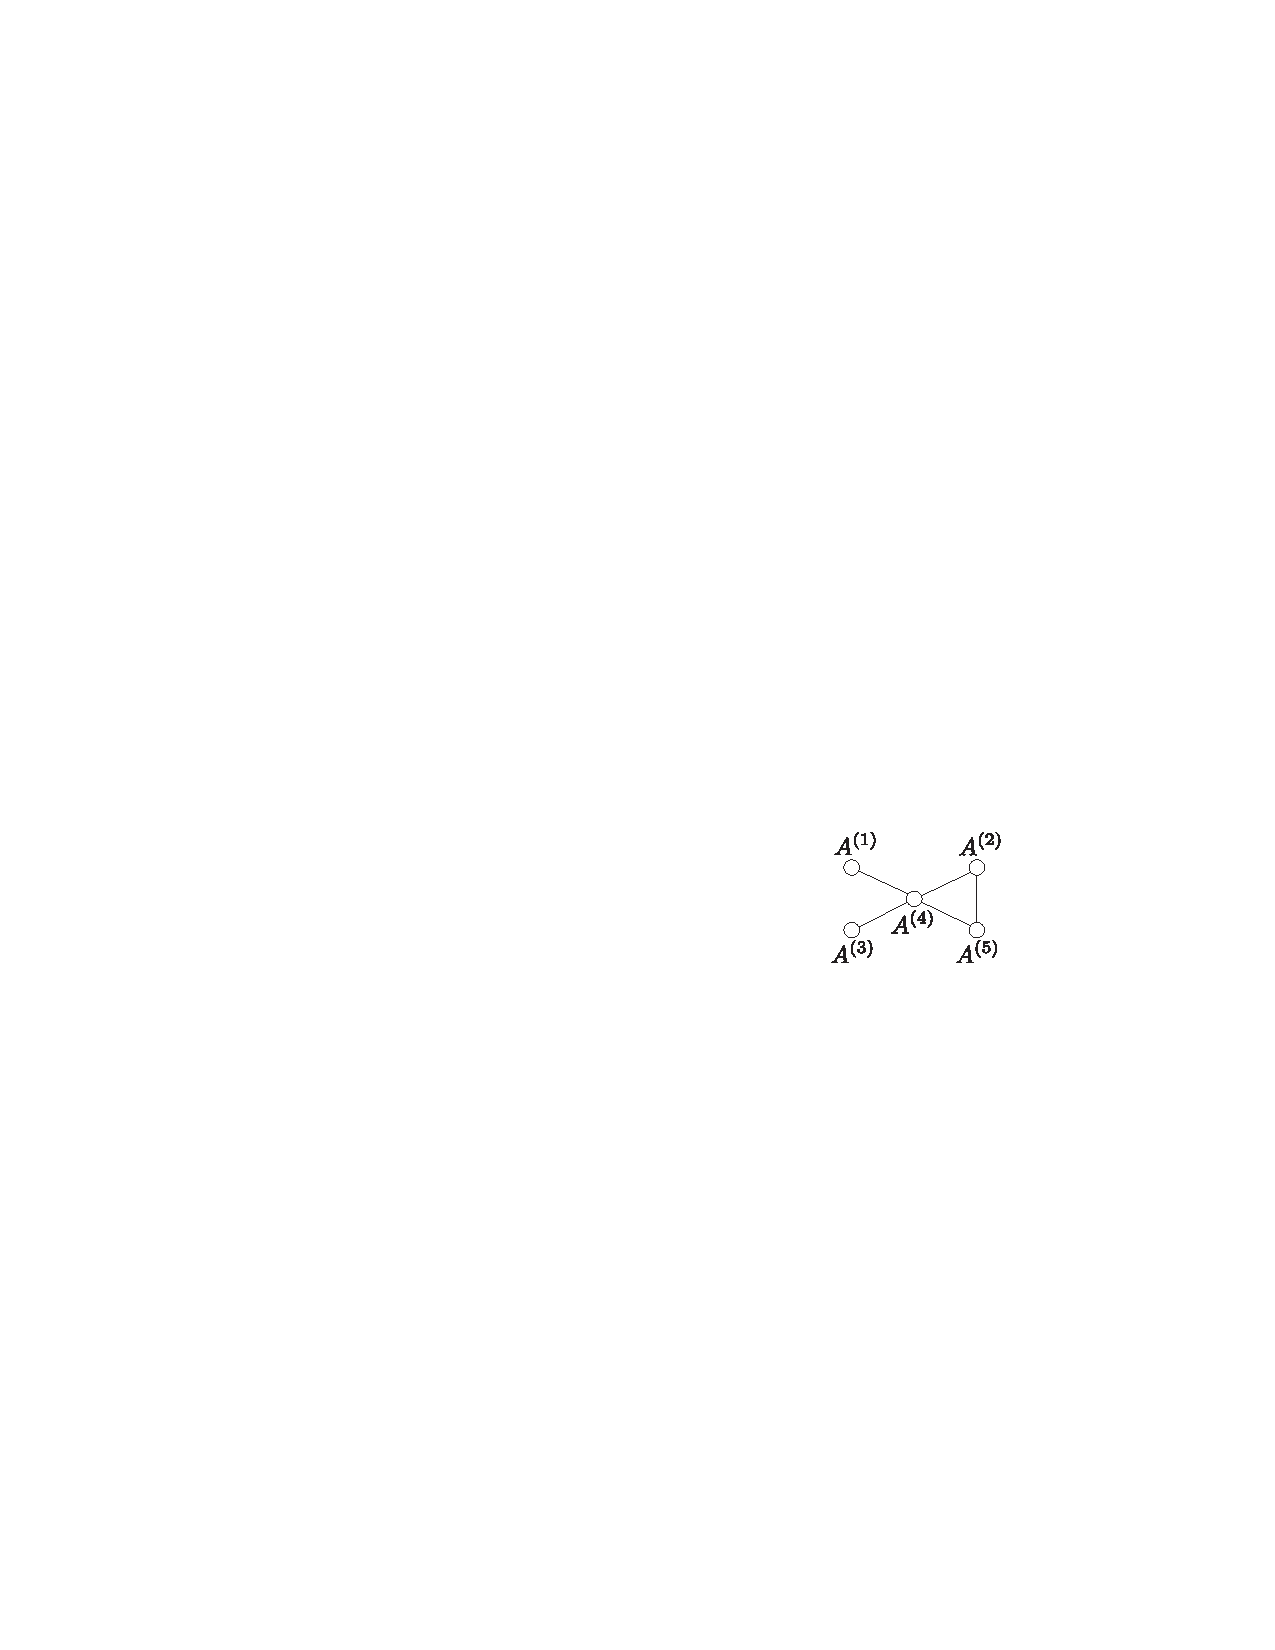
\includegraphics[width=0.4\columnwidth]{QW_arbitrary_graph}
\caption{A simple example of a quantum walk on an irregular graph structure. Associated with each vertex $x$ is an $\text{SU}(|n_x|)$ coin operator $A^{(x)}$, where $|n_x|$ is the number of neighbours to $x$.} \label{fig:QW_arbitrary_graph}\index{Quantum walk graph}
\end{figure}

The total time evolution is defined analogously to before,
\begin{align}
\hat{U}_\text{QW}(t) = (\hat{S}\hat{C})^t,
\end{align}
where \mbox{$t\in \mathbb{Z}_+$}.

With this formalism, multiple walkers are easily accommodated for simply with the addition of extra walker operators. Specifically, the $n$-walker basis states are of the form,
\begin{align}
\ket{\vec{x},\vec{c}} \propto \prod_{i=1}^n \hat{w}(x_i,c_i)^\dag \ket{0},
\end{align}
where we have ignored the normalisation factor, which is a function of the number of walkers in each basis state. Any graph topology can be represented, subject to the constraint that all $A^{(x)}$ are unitary. This implies that every vertex must have as many incoming as outgoing edges, which could be either directed or undirected, subject to this constraint.

Now the probabilities of measuring the walkers in different position configurations will be related to matrix permanents, in a similar manner to \textsc{BosonSampling}. But now the permanents will be of matrices that are functions of the set of $A^{(x)}$ matrices characterising the graph, rather than a Haar-random matrix.

It was shown by \cite{bib:RohdeMultiWalk11} that any such walk can be efficiently represented using a linear optics decomposition comprising at most $O(|V|^2)$ optical modes. Such a decomposition for \mbox{$|V|=3$} is shown in Fig.~\ref{fig:QW_LO_representation}.

\begin{figure}[!htb]
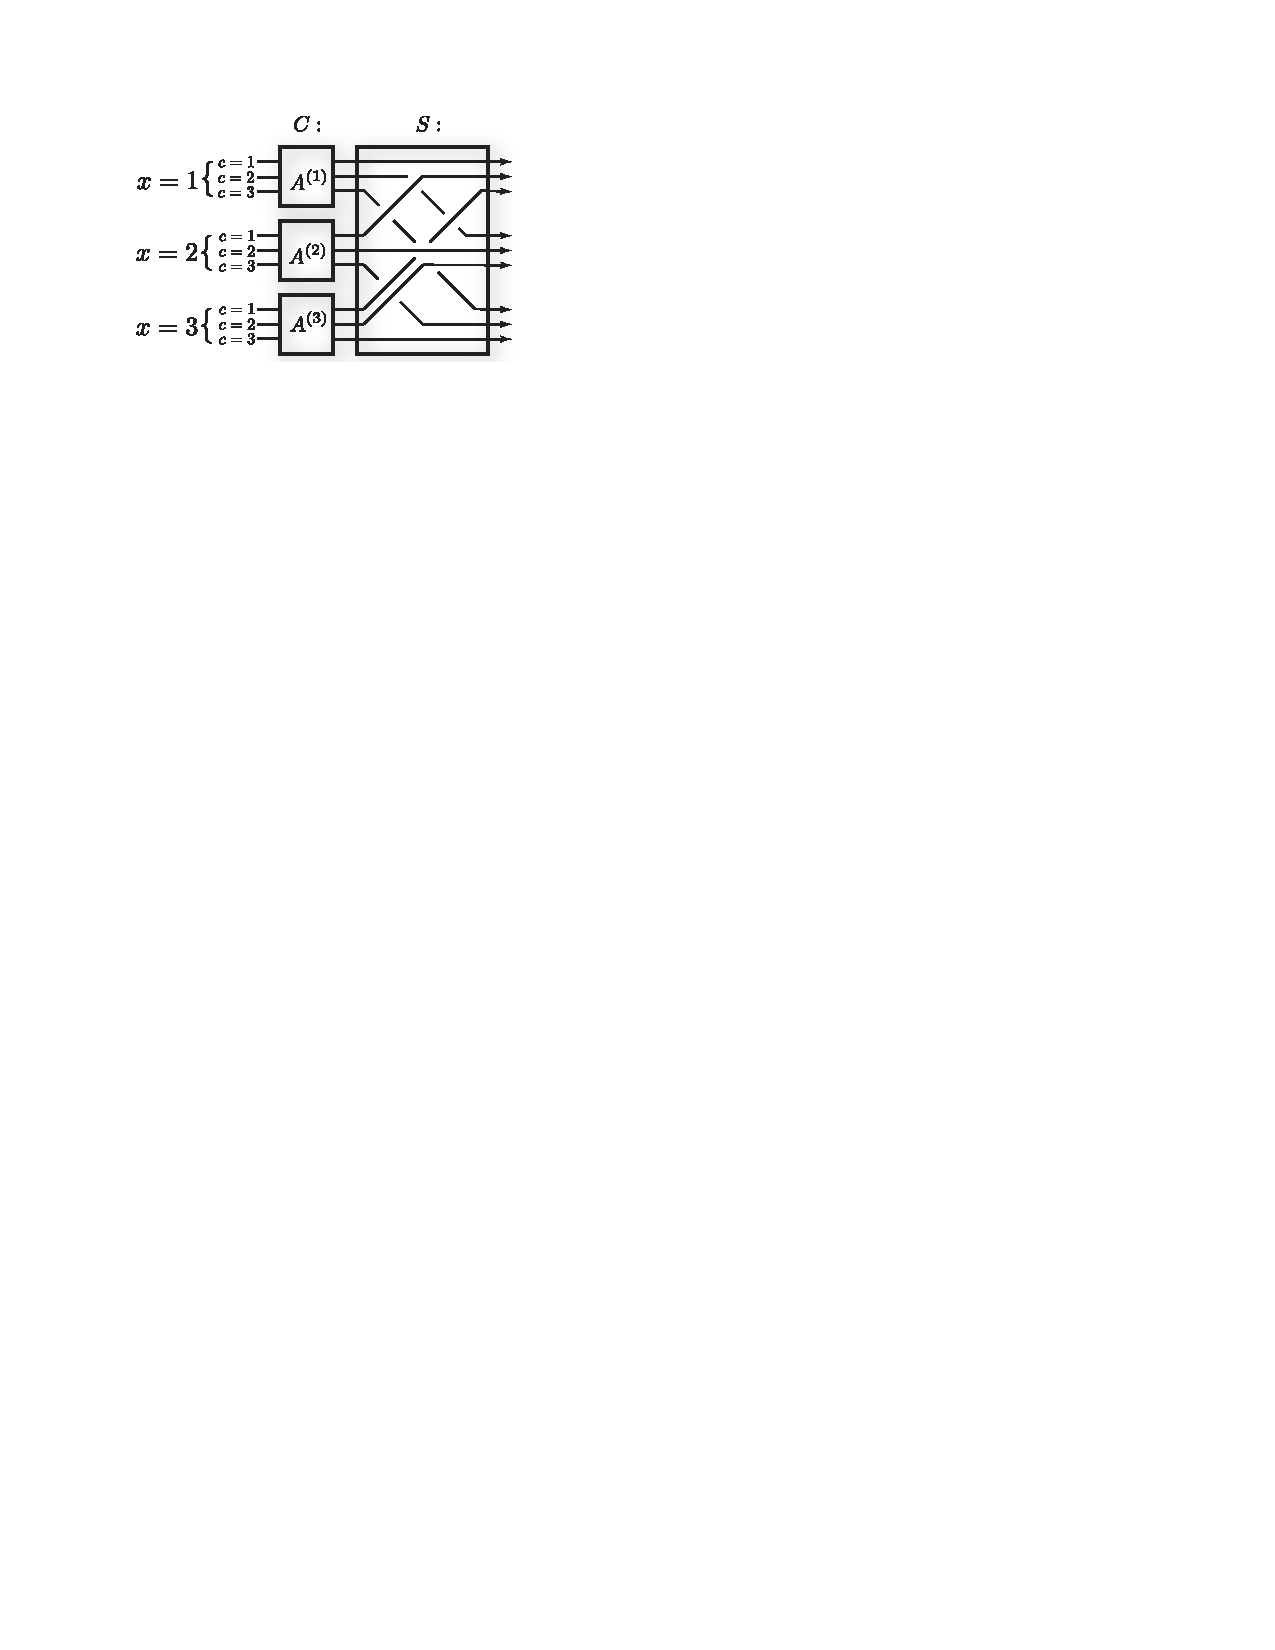
\includegraphics[width=\columnwidth]{QW_LO_representation}
\caption{Linear optics decomposition for a single step of an arbitrary 3-vertex discrete-time quantum walk. The coin operators, $A^{(x)}$, may be arbitrary $\text{SU}(3)$ matrices, whereas the step operator is simply a permutation of the optical modes. $O(|V|^2)$ optical modes are required, which scales efficiently.} \label{fig:QW_LO_representation}
\end{figure}

Because of the graph structure of the walk, it lends itself naturally to distributed implementation. We might imagine that different subgraphs -- or `widgets' \cite{bib:Lovett10, bib:Childs09} -- implement different computational primitives or subroutines. These widgets might be proprietary or expensive to implement, and are therefore best outsourced over a network.

%
% Coherent States
%

\subsubsection{Coherent states} \label{sec:coherent_state_QC} \index{Coherent state computation}

A linear optics network acting on a tensor product of coherent state inputs implements simple matrix multiplication on the vector of coherent amplitudes. Specifically, Eq.~(\ref{eq:LO_unitary_map}) implies that for the input multi-mode coherent state,
\begin{align}
\ket{\psi}_\text{in} = \ket{\vec\alpha} = \ket{\alpha_1,\dots,\alpha_m},
\end{align}
where $\alpha_i$ is the coherent amplitude of the $i$th mode, the linear map now takes the form,
\begin{align}
\beta_i = \sum_{j=1}^m U_{i,j} \alpha_j,
\end{align}
where the output state is the separable multi-mode coherent state,
\begin{align}
\ket{\psi}_\text{out} = \ket{\vec\beta} = \ket{\beta_1,\dots,\beta_m}.
\end{align}
Equivalently, this could simply be expressed as the matrix equation,
\begin{align}
\vec{\beta} = U\cdot\vec{\alpha}.
\end{align}

Of course this is not strictly a \textit{quantum} computation, since:
\begin{itemize}
\item It can be efficiently classically computed using $O(m^2)$ operations\footnote{Using the na\"ive element-wise approach, which can be further improved upon using more sophisticated contemporary algorithms.}, thus residing in \textbf{P}\index{\textbf{P} \& \textbf{BPP}}.
\item Coherent states are considered classical states (i.e laser light).
\item There is no entanglement between modes.
\item The algorithm offers no quantum speedup.
\end{itemize}

Despite offering no direct quantum advantage, we introduce this model for restricted computation, since it lends itself very elegantly to a form of homomorphic encryption, to be described in detail in Sec.~\ref{sec:homo_coherent_state}.

The applications for matrix multiplication needn't be stated, as it forms such a ubiquitous elementary primitive throughout linear algebra and in solving systems of differential equations, with applications too many to count.

%
% Continuous Variables
%

\subsection{Continuous variables (CV)} \label{sec:CV_QC} \index{Continuous variable (CV) quantum computation}

\rohit{Rohit to do}

Sec.~\ref{sec:CV_enc}
\cite{bib:Menicucci06, lund, ralph, weedbrook}
Cat states
Gaussian states

%
% Hybrid Architectures
%

\subsection{Hybrid architectures} \label{sec:hybrid} \index{Hybrid architectures}

It is unlikely that future, large-scale quantum computers will be purely optical. Some other technologies have a more favourable outlook in terms of scalability. Nonetheless, when it comes to networking quantum computers, optics is the natural approach, motivating investigation into hybrid architectures, where qubits are represented using some non-optical system, but entangling operations (EOs)\index{Entangling operations} between them are mediated by optical states and linear optics \cite{bib:Duan06, bib:Beugnon06}.

The natural example is matter qubits which couple to single-photon states, whereupon which-path erasure between coupled optical modes teleports entanglement onto the physical matter qubits.\index{Which-path erasure} Similarly, measurement of the matter qubits may be performed by stimulating the emission of photons from them. This idea has been applied to $\lambda$-configuration atomic qubits \cite{bib:BarrettKok05}, shown in Fig.~\ref{fig:barrett_kok}, and atomic ensemble qubits \cite{bib:RohdeAtEns10} (Sec.~\ref{sec:atomic_ens}). The protocol is described in Alg.~\ref{alg:which_path}.

Optically-mediated atomic ensemble quantum computing architectures are particularly attractive, as discussed in Sec.~\ref{sec:atomic_ens}\index{Atomic ensembles}.

A novel `double heralding' technique, introduced in \cite{bib:BarrettKok05}, allows loss to be overcome during which-path erasure \comment{Check this, is this what the double heralding does?}. Similarly, quantum states of light can be coupled to two-level quantum systems using Hamiltonians of the form shown in Eq.~(\ref{eq:two_level_hamil}). The preparation of long-distance entanglement between atomic systems has been demonstrated \cite{bib:Matsukevich05, bib:Matsukevich05b}

\begin{figure}[!htb]
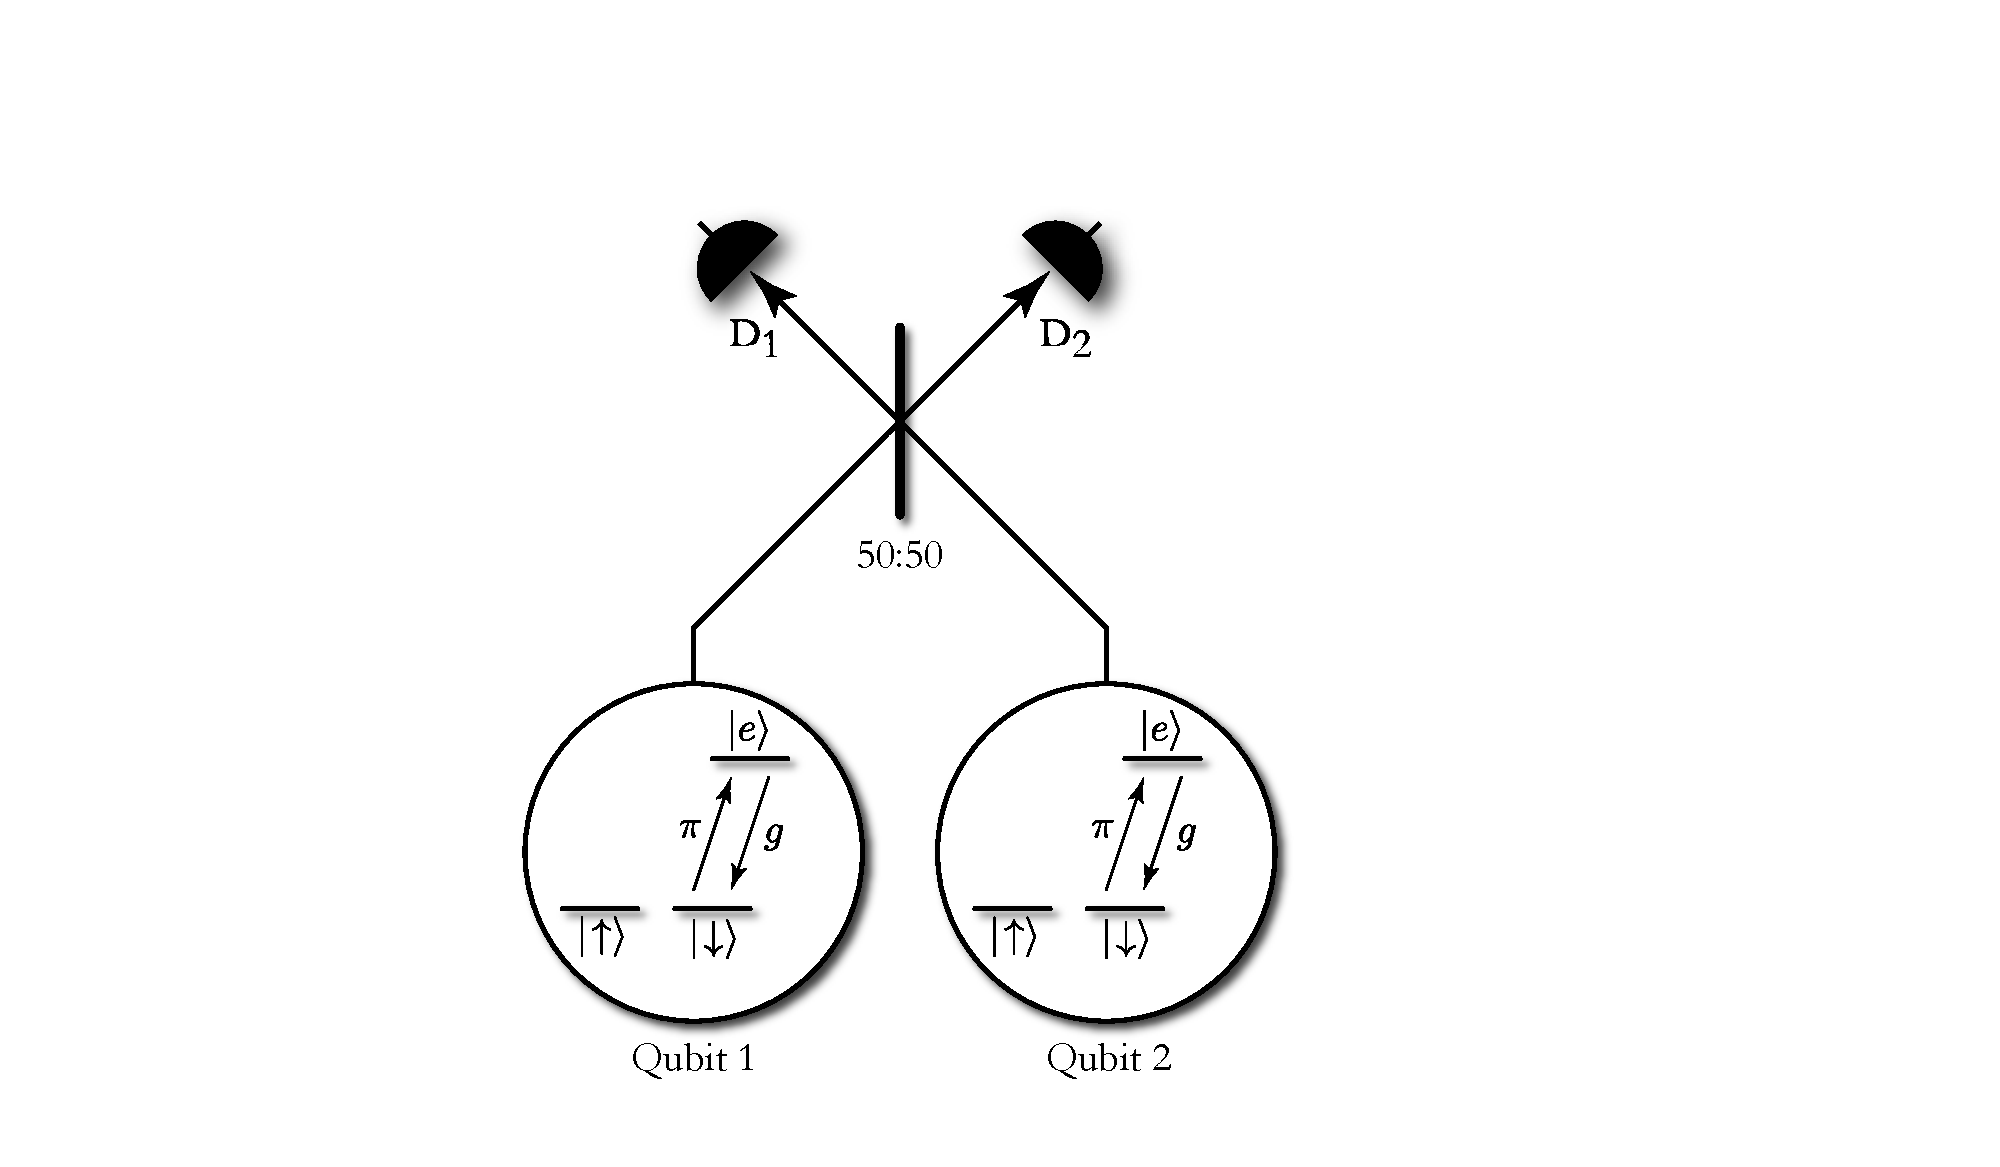
\includegraphics[width=0.75\columnwidth]{barrett_kok}
\caption{Two atomic systems in $\lambda$-configurations, each coupled with an optical mode. An EO between them is mediated via linear optics which-path erasure. Each system contains two degenerate ground states, which jointly encode a qubit (\mbox{$\ket{0}\equiv\ket{\!\uparrow}$}, \mbox{$\ket{1}\equiv\ket{\!\downarrow}$}), and an additional excited state ($\ket{e}$), which only couples to the $\ket{\!\downarrow}$ state. A $\pi$-pulse excites the electron from the $\ket{\!\downarrow}$ to the $\ket{e}$ state, after which emission of a photon is associated with a coherent relaxation back to $\ket{\!\downarrow}$. If the two optical modes are interfered on a 50:50 beamsplitter, and a single photon is detected between the two photo-detectors, $D_1$ and $D_2$, the two emission processes become indistinguishable, and which-path erasure entangles the two qubits by projecting them onto a maximally entangled Bell-pair. More complicated networks based on this EO allow the preparation of cluster states, enabling universal quantum computation. In a quantum networking context, the matter qubits could be held by a client, and the optical interferometry implementing the computation outsourced to the cloud, i.e the PBS, $D_1$ and $D_2$ are implemented in the cloud. This would also facilitate the preparation of shared entangled states, where different clients possess parts of an entangled state, potentially physically separated over long distances.} \label{fig:barrett_kok}
\end{figure}

The attractive feature of this type of approach is that the actual entanglement is generated using all-optical operations, despite the underlying logical qubits being stationary and potentially physically separated a long distance apart, mitigating the need for direct matter-matter interactions, and enabling distributed computation. Optical interfacing is discussed in Sec.~\ref{sec:opt_inter}. This allows the EOs to be performed remotely in the cloud, without physically moving the stationary qubits. Such hybrid systems present an interesting platform for cloud quantum computing -- despite the qubits being stationary, we are able to outsource the interactions between them to distant servers or even satellites.

Importantly, the beamsplitter mediating the which-path erasure EO is based upon HOM interference, and therefore does not require interferometric stability, making the outsourcing process relatively robust.

This protocol can be regarded as a variation on the entanglement swapping protocol (Sec.~\ref{sec:swapping}), whereby entanglement between matter qubits and optical modes is swapped onto entanglement between the distinct matter qubits.

Alternately, if there is no direct line of quantum communication between two qubits, an EO can be performed by directly employing the same idea in reverse. We imagine that a third party, such as a satellite, acts as a server for entangled Bell pairs. Two parties receive one qubit each from the pair. Then they perform an EO between their halves of the Bell pair and their local qubits. With appropriate local corrections, mediated by only cheap classical communication, this teleports the action of an EO onto the two qubits, creating a link between them.

Expanding upon this idea, we can envisage distributed models for quantum computation, where the qubits needn't even be of the same physical medium. We could, for example, entangle quantum dot qubits, atomic qubits, and atomic ensemble qubits with one another by coupling them to optical modes and performing which-path erasure between them. This enables distributed quantum computation between hosts possessing quantum infrastructure comprising different physical mediums (provided the photons emitted by those systems may be made indistinguishable, such that HOM interference is possible).

\begin{table}[!htb]
\fbox{\parbox{0.965\columnwidth}{\texttt{ 
function WhichPathErasure():
\begin{enumerate}
\item Alice and Bob each prepare an equal superposition of the two logical basis states,
\begin{align}
\ket\psi_\text{in} = &\frac{1}{2}(\ket{\!\uparrow}_{A_1}+\ket{\!\downarrow}_{A_1})\ket{0}_{A_2}\nonumber \\
&\cdot (\ket{\!\uparrow}_{B_1}+\ket{\!\downarrow}_{B_1})\ket{0}_{B_2},
\end{align}
where $A_1/B_1$ denote the matter qubits, and $A_2/B_2$ denote their coupled optical modes.
\item Apply a $\pi$-pulse to each qubit, inducing a \mbox{$\ket{\!\downarrow}\to\ket{e}$} transition,
\begin{align}
\ket\psi_\pi = \hat{U}_\pi\ket\psi_\text{in} = &\frac{1}{2}(\ket{\!\uparrow}_{A_1}+\ket{e}_{A_1})\ket{0}_{A_2}\nonumber \\
&\cdot (\ket{\!\uparrow}_{B_1}+\ket{e}_{B_1})\ket{0}_{B_2}.
\end{align}
\item Wait for a coherent relaxation, inducing the transition \mbox{$\ket{e}\to\ket{\!\downarrow}\hat{a}^\dag$}, which emits a single photon,
\begin{align}
\ket\psi_\text{relax} = \hat{U}_\text{relax}\ket\psi_\pi = &\frac{1}{2}(\ket{\!\uparrow}_{A_1}+\ket{\!\downarrow}_{A_1}\hat{a}^\dag_{A_2})\ket{0}_{A_2}\nonumber \\
&\cdot (\ket{\!\uparrow}_{B_1}+\ket{\!\downarrow}_{B_1}\hat{a}^\dag_{B_2})\ket{0}_{B_2}.
\end{align}
\item Apply a 50:50 beamsplitter between the two optical modes,
\begin{align}
\ket\psi_\text{BS} = \hat{U}_\text{BS} \ket\psi_\text{relax} = &\frac{1}{2}(\ket{\!\uparrow}_{A_1}+\ket{\!\downarrow}_{A_1}[\hat{a}^\dag_{A_2}+\hat{a}^\dag_{B_2}])\nonumber \\
&\cdot (\ket{\!\uparrow}_{B_1}+\ket{\!\downarrow}_{B_1}[\hat{a}^\dag_{A_2}-\hat{a}^\dag_{B_2}])\nonumber \\
&\cdot \ket{0}_{A_2}\ket{0}_{B_2}.
\end{align}
\item Conditional upon detecting exactly one photon between the output optical modes, we obtain,
\begin{align}
\ket\psi_\text{out}^{1,0} = \bra{1,0}_{A_2,B_2} \ket\psi_\text{BS} = \frac{1}{2} (\ket{\!\uparrow,\downarrow}_{A_1,B_1} + \ket{\!\downarrow,\uparrow}_{A_1,B_1}), \nonumber \\
\ket\psi_\text{out}^{0,1} = \bra{0,1}_{A_2,B_2} \ket\psi_\text{BS} = \frac{1}{2} (\ket{\!\uparrow,\downarrow}_{A_1,B_1} - \ket{\!\downarrow,\uparrow}_{A_1,B_1}),
\end{align}
which is a Bell-pair between the matter qubits.
\end{enumerate}}}}
\caption{Using which-path erasure to entangle two $\lambda$-configuration matter qubits via post-selected linear optics. Note that the two matter qubits could in principle be arbitrarily physically separated. Only the emitted photons need be brought together locally for the implementation of a beamsplitter operation. This lends such entanglement generation protocols to distributed implementation.} \label{alg:which_path}
\end{table}